\chapter{Numerical Simulations of Stenotic Flow}

Peripheral arterial occlusive diseases, especially in femoral arteries are commonly seen by clinical doctors in the U.S.\cite{malinow1989prevalence, boger1997biochemical, hooi2001incidence}. These patients may have critical stenoses or multiple sequential moderate stenoses. The current clinical practice usually recommends simple balloon angioplasty\cite{duncan1995simple} to treat critical stenotic lesion, i.e. $ > 60 \% $ luminal area reduction. However, it is a difficult process for the doctors to make a decision on whether or not to treat multiple sequential moderate stenoses using the stent or balloon angioplasty. This is partially because of the lack of methods to measure how these multiple stenoses affect their downstream blood flow. The scientific study of fluid dynamics associated with multiple stenoses is far less than that of a single stenosis. To assist on making clinical decision for treating multiple stenoses, a quantitative approach, for instance, the computational fluid dynamics (CFD) \cite{ferziger1997computational} method is very much needed. In this study,  we present a high-fidelity CFD simulations of the blood flow in the stenotic arteries using idealized geometries. We solve unsteady incompressible Navier-Stokes equations\cite{temam1984navier} using unstructured meshes with all hexahedral elements. The upstream flow condition is prescribed which gives a Reynolds number of 500. Our simulations results reveal several new discoveries of fluid dynamics in these multiple stenoses considering a range of different geometric parameters.

\section{Background}

Peripheral arterial occlusive disease are the major cause of amputation in the U.S. as they are prevalent among smokers, diabetics, hypertensives, and patients with dyslipidemia. Nowadays, since the disease can be visualized as areas of stenosis or occlusion on a diagnostic arteriogram, simple balloon angioplasty with or without stenting is usually recommended for treating critical stenotic lesions, i.e. $ > 60\% $ (by area) luminal reduction. However, the clinical decision is rather difficult on whether or not to treat subcritical stenotic lesions, i.e., $ < 50\% $ luminal reduction, in particular, multiple sequential moderate stenoses. The risks of routine ballloon angioplasty/stenting include intimal injury-induced acute arterial thrombosis or restenosis\cite{holmes1984restenosis} from neointimal hyperplasia\cite{kornowski1998stent}, etc. These risks led to the difficulty of telling the benefits of treating mildly stenotic lesions using routine clinical treatment. Meanwhile, there is no existing method to measure the effects of multiple sequential moderate stenoses on blood flow in the part of the artery that is downstream of the stenotic lesions. The closest measurement that correlated with change in blood flow is the change in arterial pressures. If the arterial pressure drop across the stenoses is greater than the clinical threshold (20-30mmHg) \cite{meuwissen2002hyperemic}, the lesions are considered physiologically significant enough to favor treatment. However, it's clinically very difficult to quantify. Consequently, CFD simulation is a helpful supplement for the stenosis study.

\begin{figure}[H]
	\centering
	\begin{tabular}{c}
		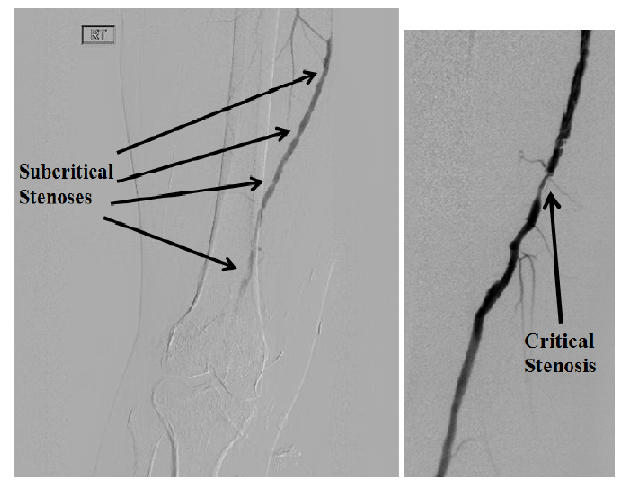
\includegraphics[width=0.6\textwidth]{./pics/photo.png}
	\end{tabular}
	\caption{\footnotesize Contrast of subcritical and critical stenoses.}
	\label{fig: patient CT}
\end{figure}

A good amount of investigation have been addressed on pressure drop across single stenosis from both experimental and analytical perspective\cite{Ojha,Varghese,Young&Tsai,Young&Cholvin,Seeley&Young,Varghese&Frankel}. At the beginning, investigators derived empirical function from conservation equations with the experimental coefficients for both steady and pulsatile flow condition. The empirical function is a simplified estimation for pressure drop across single stenosis. A series computational simulations and experiments rendered the details of flow field across constriction. 
Flanigan et al\cite{flanigan1977multiple} conducted a series of experiments and proposed non-linear relationship between number of applied stenoses and pressure drop across the stenoses.
Bertolotti et al\cite{bertolotti2006influence}, using finite element method, simulated the pressure drop and velocity field through two adjacent stenoses at very low Reynolds number.

We have implemented an efficient in-house CFD package which has the capability to simulate more complex 3D geometries. This paper reports a range of parametric studies including varying the number of stenoses, the narrowing degrees, the shapes, and streamwise spacing. The object is providing to doctors an accessible effective approach which can predict the pressure and the velocity field of stenotic arteries. These stenotic arteries consist of patient-specific geometries which are challenging to define computationally. These arteries are typically simplified as axisymmetric constriction in straight tubes. The 3D computational domain is represented by unstructured meshes with all hexahedral cells. An efficient pressure-based Finite Volume Method(FVM)\cite{LiangFVM} was implemented to solve these equations. Our simulations include computational geometries with a wide range of narrowing degrees of stenoses, from $ 40\% $ to $ 80\% $ luminal area reduction. The number of stenoses ranges from $ 1 $ to $ 7 $. Several different spatial intervals were considered between adjacent stenoses.
%=========================================

\section{Numerical Method}

The unsteady incompressible Navier-Stokes equations, describing the conservation of mass and momentum in the computational region, are discretized using a second-order central differencing scheme in space and a Crank-Nicolson\cite{briley1977solution} method in time. 
The pressure and velocity are stored in cell centers using the collocated method.
Pressure-velocity coupling is dealt by a Rhie-Chow interpolation method\cite{Rhie} and a PISO algorithm for pressure correction\cite{Issa}.

Mass conservation and Navier-Stokes equations as following:s

\begin{equation}
\frac{\partial u_{i}}{\partial x_{i}} = 0,
\end{equation}

\begin{equation}
\frac{\partial u_{i}}{\partial t} + \frac{\partial u_{i} \partial u_{j}}{\partial x_{j}} = -\frac{1}{\rho} \frac{P}{\partial x_{i}} - \frac{\partial \tau_{ij}}{\partial x_{j}} + \nu \frac{\partial^{2} u_{i}}{\partial x_{j} \partial x_{i}},
\end{equation}

where the index $ i = 1, 2, 3 $ represents three directions in the Cartesian coordinate system, $ P $ is the pressure, $ \rho $ is density, and $ \nu $ is kinematic viscosity.

\section{Geometry and Condition}

\subsection{Geometry}

The geometry of stenoses along peripheral artery is complex and irregular. A symmetrical constriction in a straight cylindrical tube is a proper idealization method to simplify the complicated problem\cite{Long}. The shape of the stenoses are optimized by using third order degree polynomial. In the following figure shows three sequential $ 50\% $ degree stenoses along the straight vessel.

\begin{figure}[H]
	\centering
	\begin{tabular}{c}
		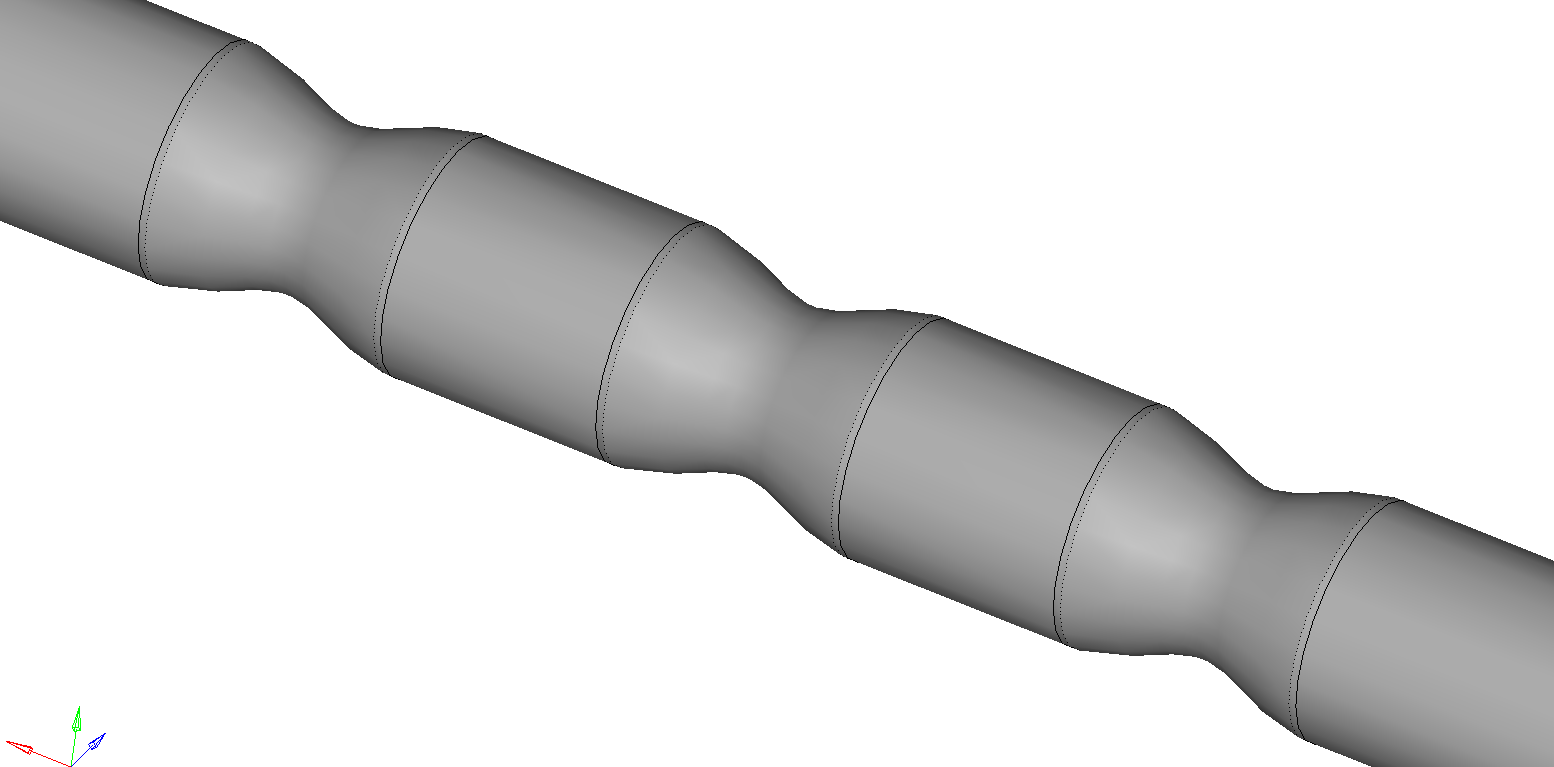
\includegraphics[width=0.6\textwidth]{./pics/geom.png}
	\end{tabular}
	\caption{\footnotesize Geometry of sequential stenoses.}
\end{figure}

\subsection{Mesh}
We implement unstructured hexahedral meshes for idealized stenoses geometry. Internal mesh is total unstructured as the following figure. Moreover, we impose flour boundary layers along the surrounding wall for more accurate prediction of boundary flow.

\begin{figure}[H]
	\centering
	\begin{tabular}{cc}
		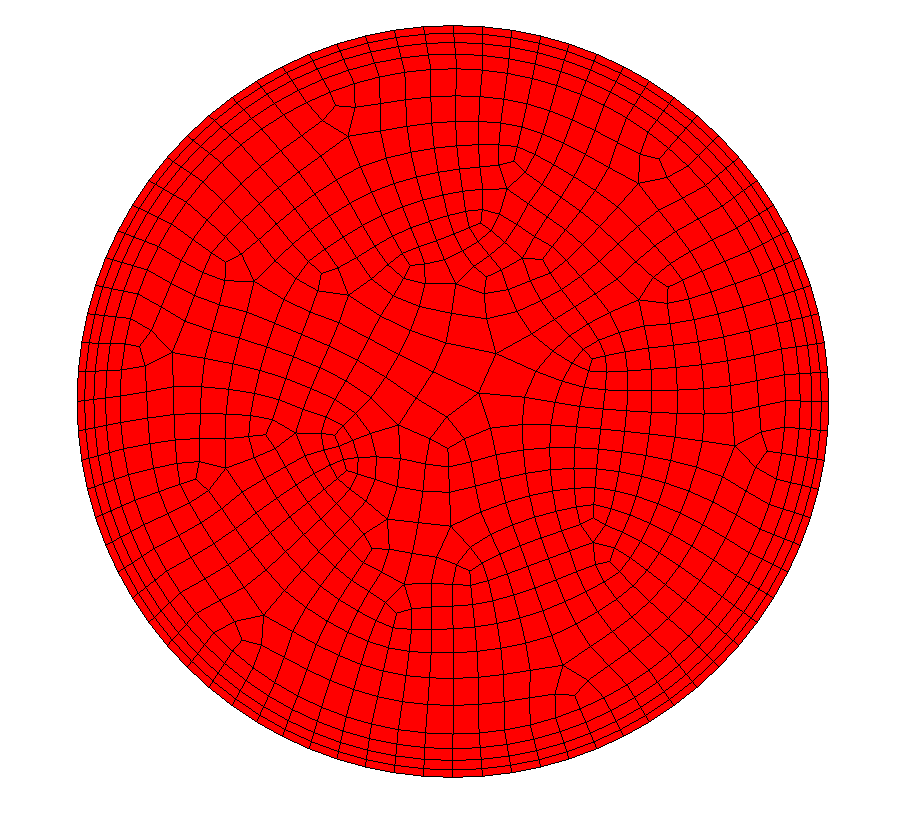
\includegraphics[width=0.3\textwidth]{./pics/mesh1.png} & 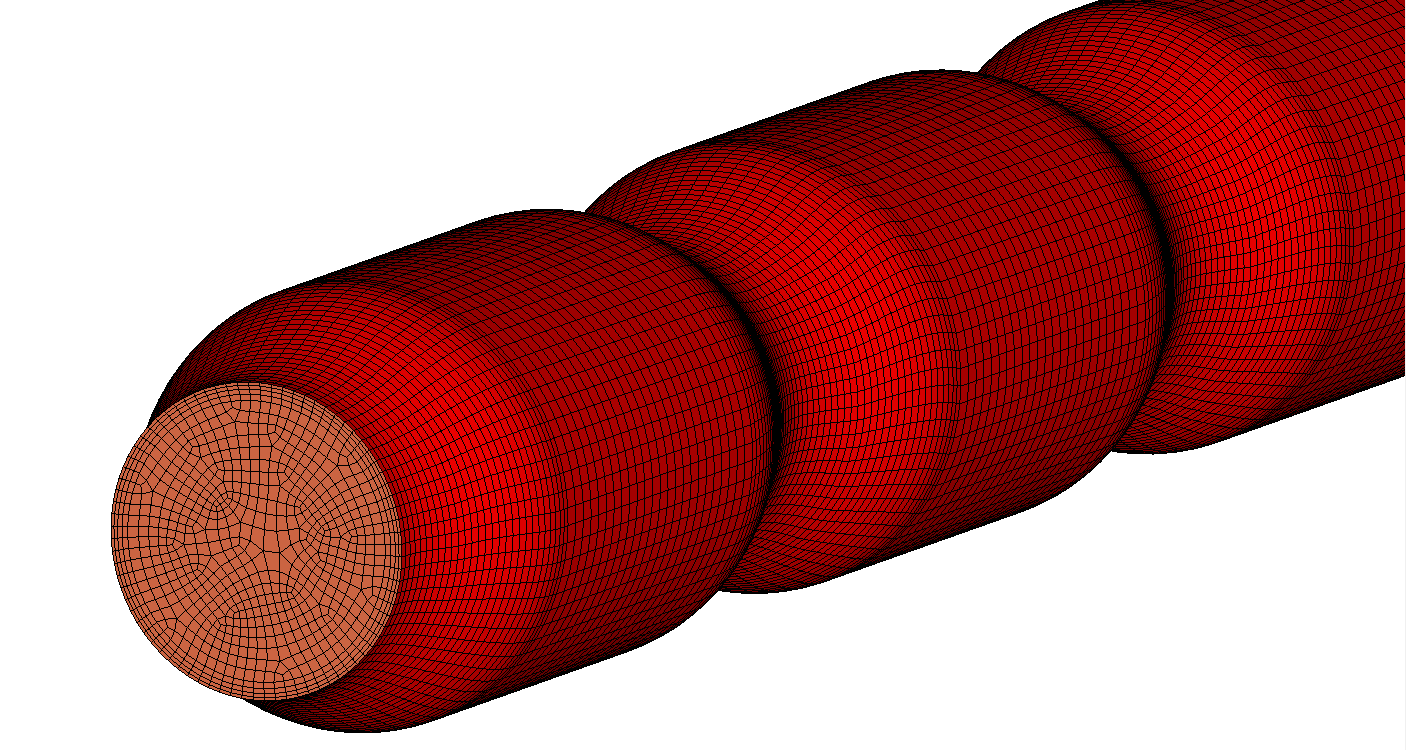
\includegraphics[width=0.6\textwidth]{./pics/mesh7.png}
	\end{tabular}
	\caption{\footnotesize Cross-sectional view of hexahedral meshes.}
\end{figure}

To better analyze the flow cross the stenotic area, we refine the longitudinal mesh across the stnosis. We increase the number of layers along x-axis direction for a better mesh adaptation of stenosis curve.

\begin{figure}[H]
	\centering
	\begin{tabular}{cc}
		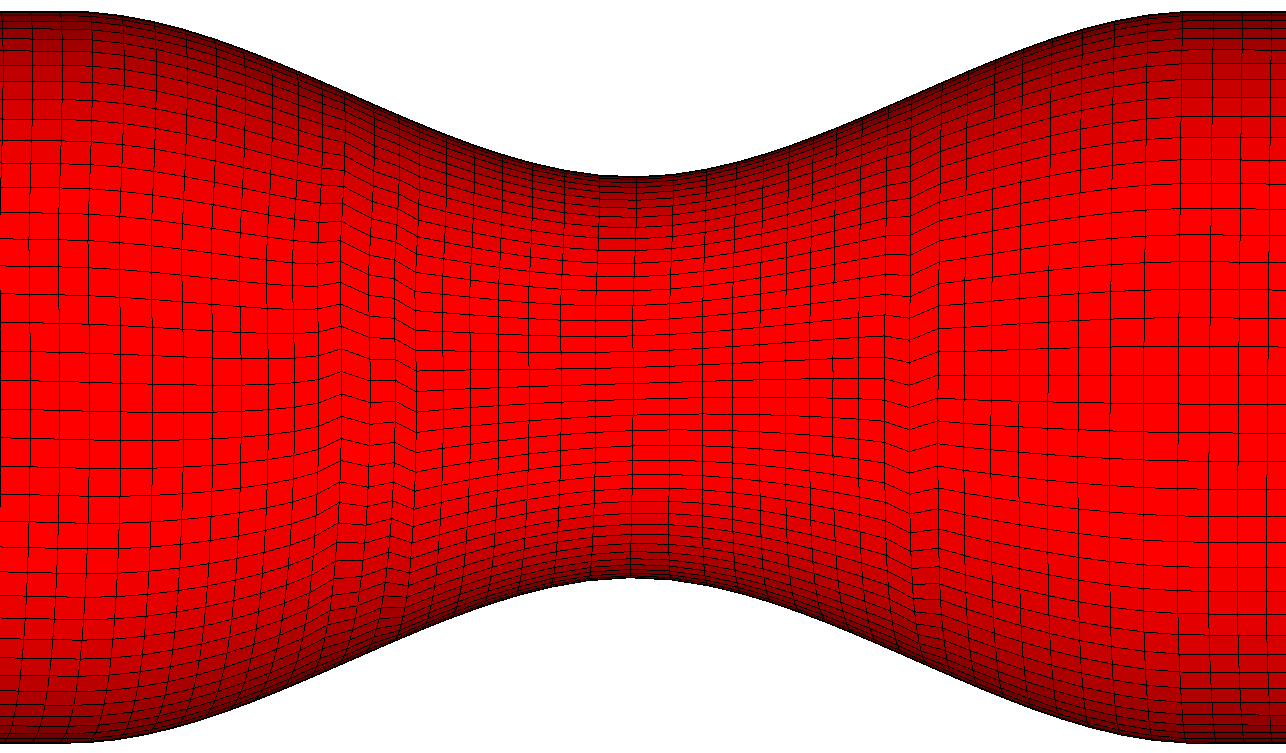
\includegraphics[width=0.4\textwidth]{./pics/refine1.png} & 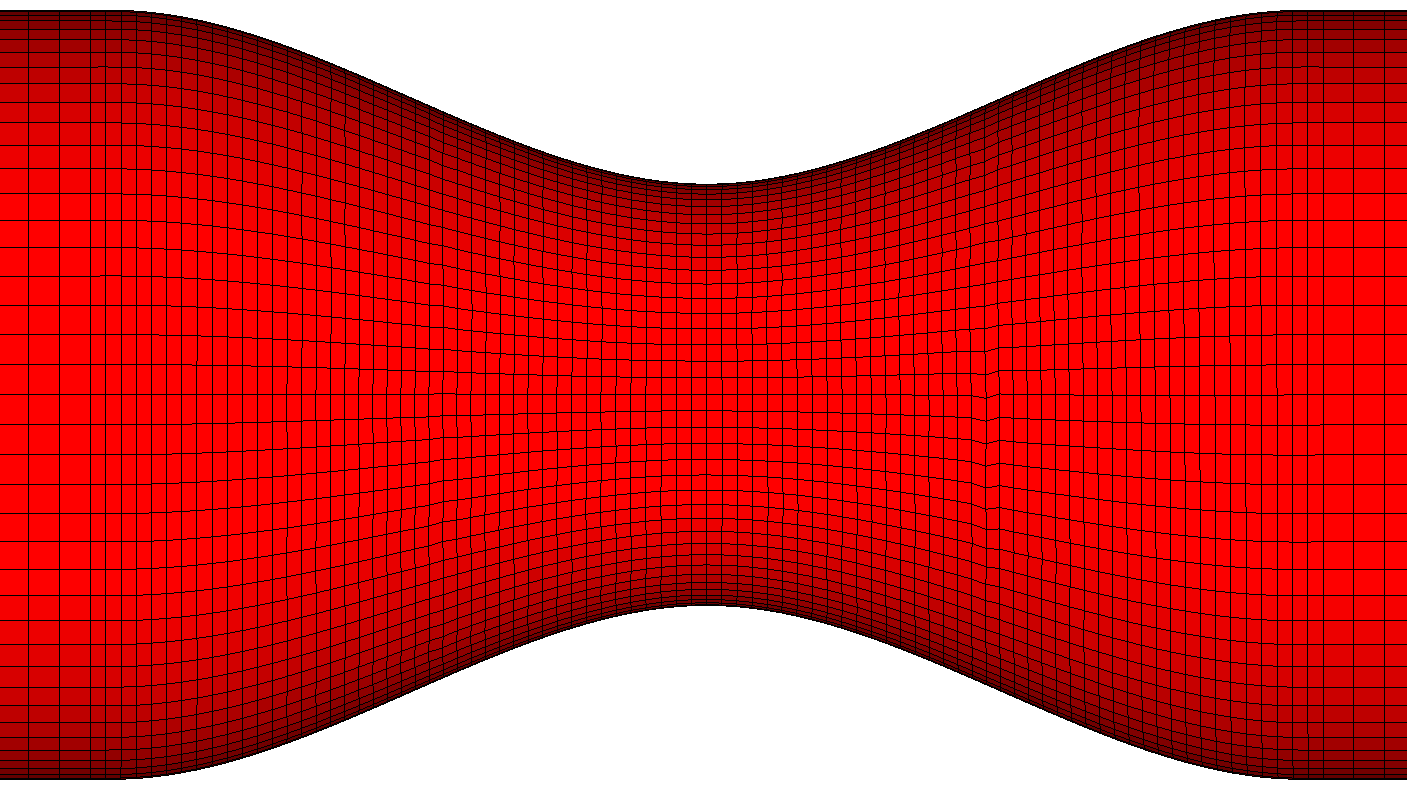
\includegraphics[width=0.4\textwidth]{./pics/refine2.png}
	\end{tabular}
	\caption{\footnotesize Mesh refinement for stenotic area.}
\end{figure}

\subsection{Dimensionless wall distance}

The transition flow happens when the flow passing critical (i.e. $ >70\% $) stenosis. The dimensionless wall distance is defined as:

\begin{equation}
y^{+} = \frac{u_{*} y}{\nu}
\end{equation}

where $u_*$ is the friction velocity at nearest wall, $y$ is the distance to the nearest wall,$\nu$ is the local. kinematic viscosity of fluid. 
We control the $y^+ \le 1$ after refine the mesh with boundary layers. This condition insure that viscosity plays an important role rather than advection.

\subsection{Conditions}

	\begin{table}[!h]
		\caption{ Simulation condition parameters.}
		\vspace{-5pt}
		\begin{center}
			%	\scalebox{0.6}{
			\begin{tabular}{|c|c|}
				\hline
				\textbf{Variable} &\textbf{Value}\\
				\hline
				Stream wise length & 30D\\
				\hline
				Reference mesh points & 720,000\\
				\hline
				Reynolds number for inlet & 500\\
				\hline
				Maximum of CFL number & 0.79\\
				\hline
			\end{tabular}
			%	}
		\end{center} 
	\end{table}

	We implement parabolic velocity profile as inlet boundary condition, Neumann condition as the outlet boundary condition.
	We impose no-slip boundary condition on rigid and non-porous walls.
	The fluid is incompressible Newtonian with same mean Reynolds number as blood in peripheral arteries ${Re}_{mean} = 500$.
	The entrance length of 6 diameters is sufficient for flow development.

%=========================================

\section{Verification}
\subsection{Straight vessel test}
First of all, we implement a simulation on a straight tube without any constriction.
For the straight tube, we use the following analytical function to calculate the pressure drop
\begin{equation}
\Delta P  = \frac{128 \mu l Q}{\pi D^4}
\end{equation} 
We compare the pressure drop between simulation results and analytical solution. The error is less than $0.25$\%.

\begin{table}[h]
	\caption{ Straight vessel test results.}
	\vspace{-5pt}
	\begin{center}
		%	\scalebox{0.6}{
		\begin{tabular}{|c|c|}
			\hline
			\textbf{Cases} &\textbf{Value}\\
			\hline
			Simulation result & 408.6 \\
			\hline
			Analytical solution & 409.9 \\
			\hline
			Error & $<0.25$\% \\
			\hline
		\end{tabular}
		%	}
	\end{center} 
\end{table}

For the following cases, we use the value of pressure drop through the straight tube as a reference bar.
All the parameters including absolute and stream-wise pressure drop are plotted over the reference value.
The coordinate information are plotted over the diameter.
Then all the parameters on the following figures are dimensionless.

\subsection{Resolution independence test}

In this section, we present the results of same geometry with two different mesh resolutions.
The test cases are straight tubes with 10 diameters long. 

\begin{figure}[H]
	\centering
	\begin{tabular}{cc}
		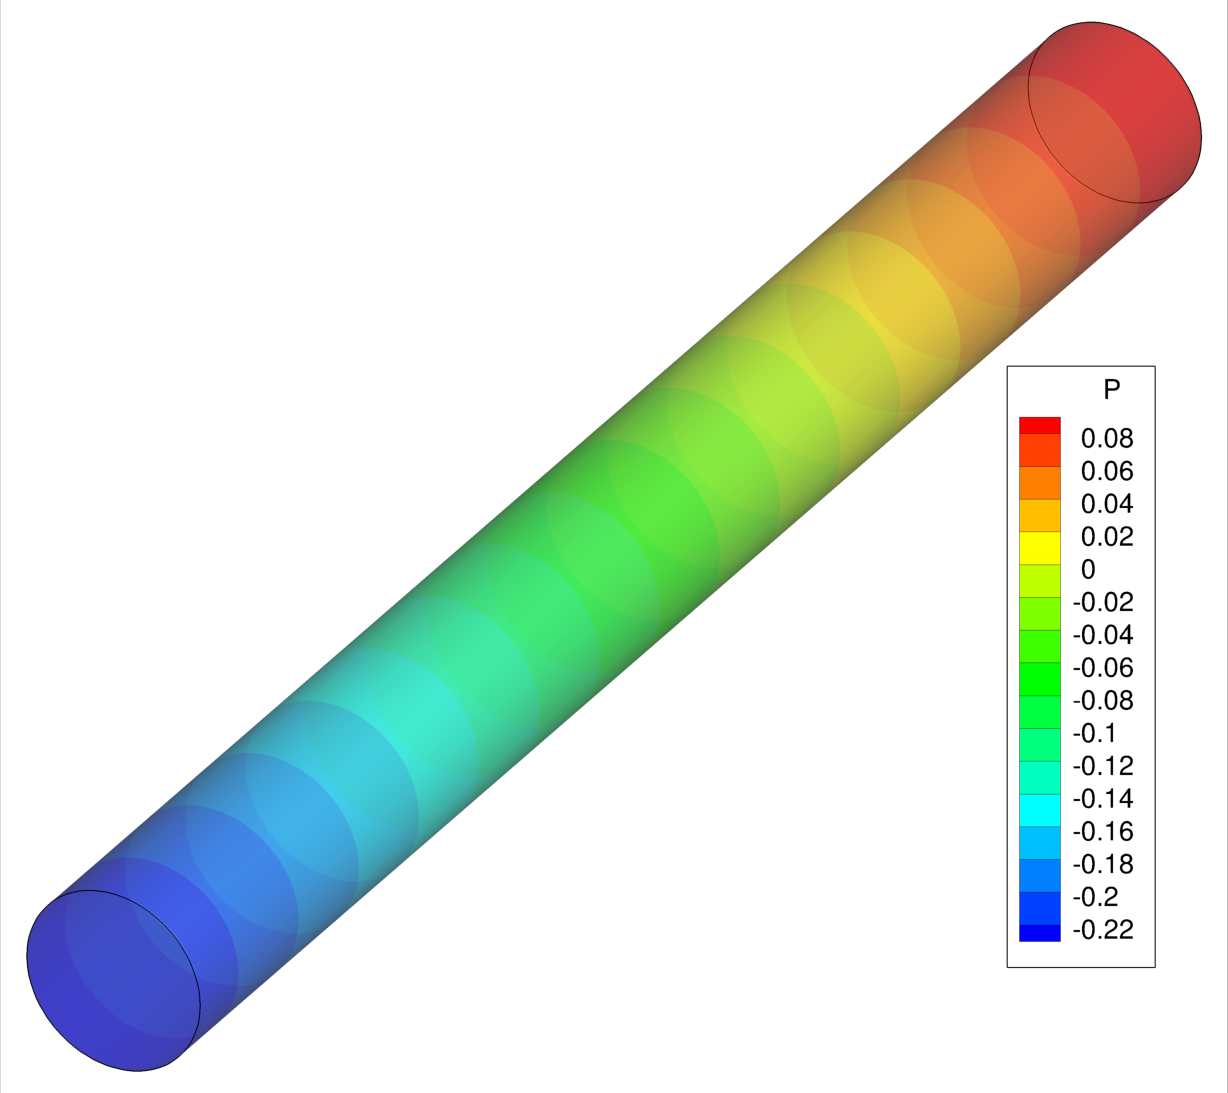
\includegraphics[width=0.4\textwidth]{./pics/plotbio.png} & 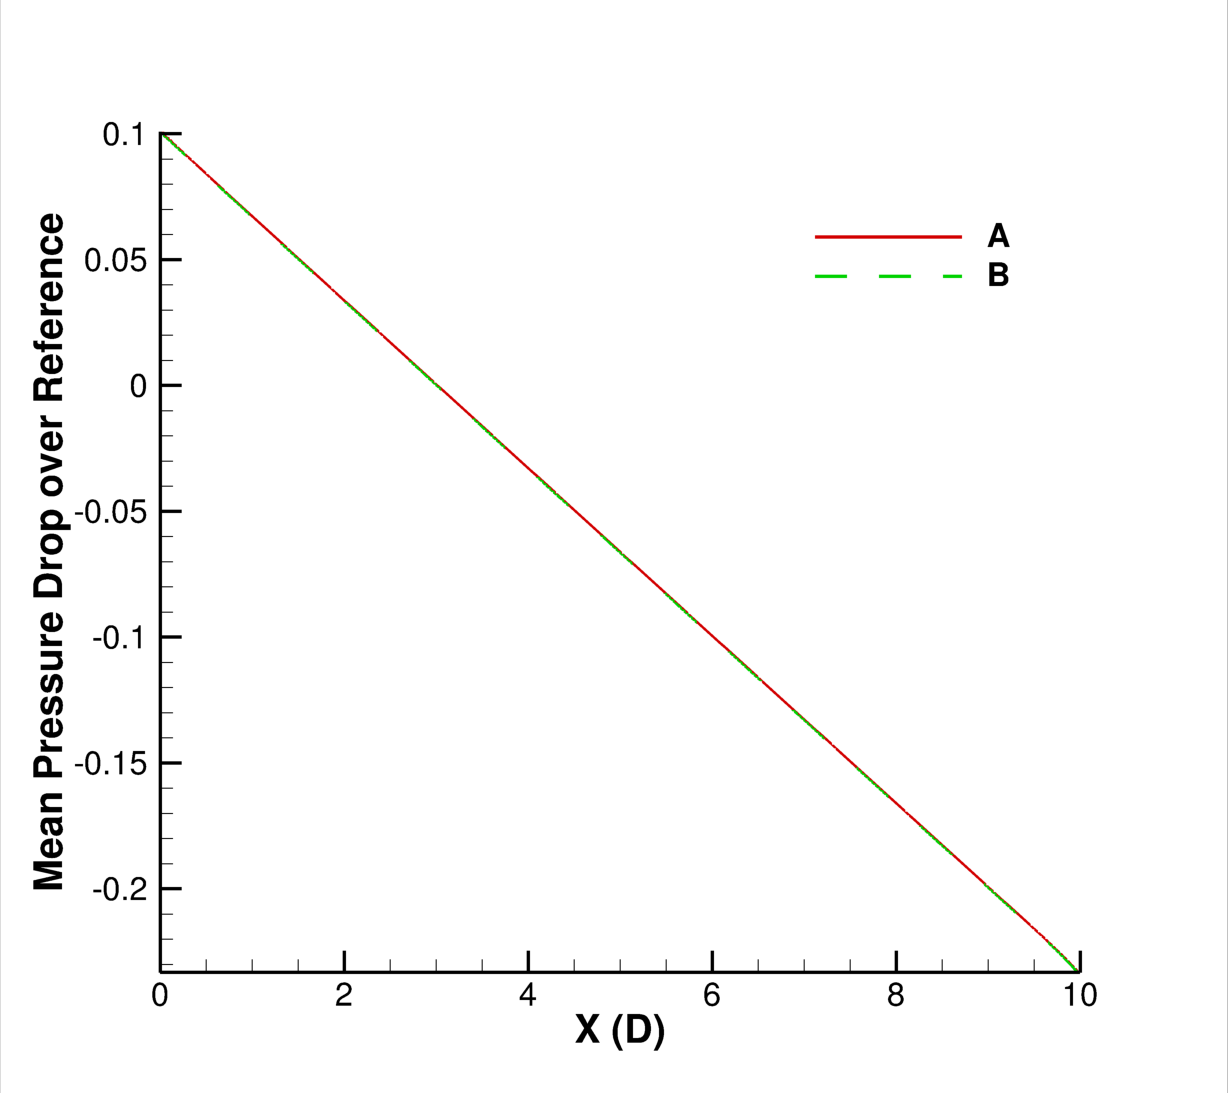
\includegraphics[width=0.4\textwidth]{./pics/resolution.png}
	\end{tabular}
	\caption{\footnotesize Resolution independence test plot and results comparison.}
\end{figure}

The reference mesh grids number of case A is 240000. The resolution of case A is as same as the rest simulations of this paper. We double the number of mesh grid along the longitudinal direction. The finer mesh case B has 480000 grid points. Then we simulate both cases with our solver and compare the results with analytical solution.

\begin{table}[h]
	\caption{Resolution independence test results.}
	\vspace{-5pt}
	\begin{center}
		%	\scalebox{0.6}{
	\begin{tabular}{|c|c|c|}
		\hline
		\textbf{Cases} &\textbf{Value} & \textbf{Error}\\
		\hline
		A & 136.946 & $<0.57\%$\\
		\hline
		B & 137.211 & $<0.76\%$\\
		\hline
		Analytical & 136.169 & 0 \\
		\hline
	\end{tabular}
		%	}
	\end{center} 
\end{table}

The error of both cases are very low and neglectable. The resolution of case A is same as all the simulations in this paper. From this comparison we can conclude that our resolution is sufficient for pipe-flow study. It is a good compromise on accuracy and efficiency of simulations.

%===================================================
\section{Results}

To analyze the hemodynamic effect caused by variant stenoses, we introduced two key parameters which describe the pressure field through stenotic artery. 
The first one is the  stream-wise pressure drop which indicates the pressure difference from the inlet to the outflow area through the whole arterial domain.  
It describes the hemodynamic effect of stenoses among the entire flow domain. The doctors currently are using it as a prime clinical indicator to evaluate blood supplement to downstream bodies. Doctors are using this parameter to make the treatment decision.
The other one is the absolute pressure drop which means the pressure difference between the maximum pressure value (at the inflow area) and minimum pressure value (at the last post-stenotic area). 
This parameter demonstrates the stenotic lesion induces a low pressure field concentrated at the post-stenotic area. 
The certain low pressure flow area is a potential serious damage source to the blood vessels which may leads to restenosis after the treatment. 

\subsection{Verification Empirical Solution}

In Young and Tsai\cite{Young&Tsai} study, the major factors controlling the pressure drop, $\triangle p$, across a single stenosis can be estimated from the following empirical equation:

\begin{equation}
\triangle p = \frac{K_v \mu}{D} U + \frac{K_t}{2}(\frac{A_0}{A_1} -1)^2 \rho \lvert U \rvert U %+ K_u \rho L \frac{dU}{dt}
\end{equation}
where $A_0$ = area of the unobstructed tube, $A_1$ = minimum cross-sectional area of the stenosis,
$D$ = unobstructed tube, $K_v$ and $K_t$ = experimentally determined coefficients, 
$L$ = length over which the pressure drop is measured, $U$ = instantaneous velocity in the unstructed tube,
$\rho$ = blood flow density, and $\mu$ = blood flow viscosity. 

Young et al\cite{Young&Cholvin} pointed out that $K_v$ and $K_t$ are dependent on stenosis geometry and narrowing degree.
$K_v$ can be approximated from steady-flow tests with streamlined plug as single stenosis.
The values of $K_v$ in our simulations range from 630 to 2300 of the stenosis narrowing degree from 40\% to 80\% area reduction.
Another empirical coefficient, $K_u$, gives the best fit of data is 1.2.

\begin{figure}[H]
	\centering
	\begin{tabular}{c}
		\includegraphics[width=0.8\textwidth]{./pics/ana3.png}
	\end{tabular}
	\caption{\footnotesize Pressure drop after single stenosis results from analytic equation and simulation.} \label{fig: single verification}
\end{figure}

In an effort to obtain the theoretic solution, we calculated the pressure drop introduced by single subcritical and critical stneosis with using equation (4).
The parameters including diameters, Reynolds number, viscosity, density and reduction area degrees are all identical for both analytical calculations and computational simulations.
We plot the pressure drop introduced from single stenosis ranges from 40\% to 80\% stenotic narrowing degrees.
The absolute pressure drop marker from simulations are very close to the theoretic calculations. 
The average error between two sets of values are less than 20\%. 


\subsection{Single stenosis evaluation}

\begin{figure}[H]
	\centering
	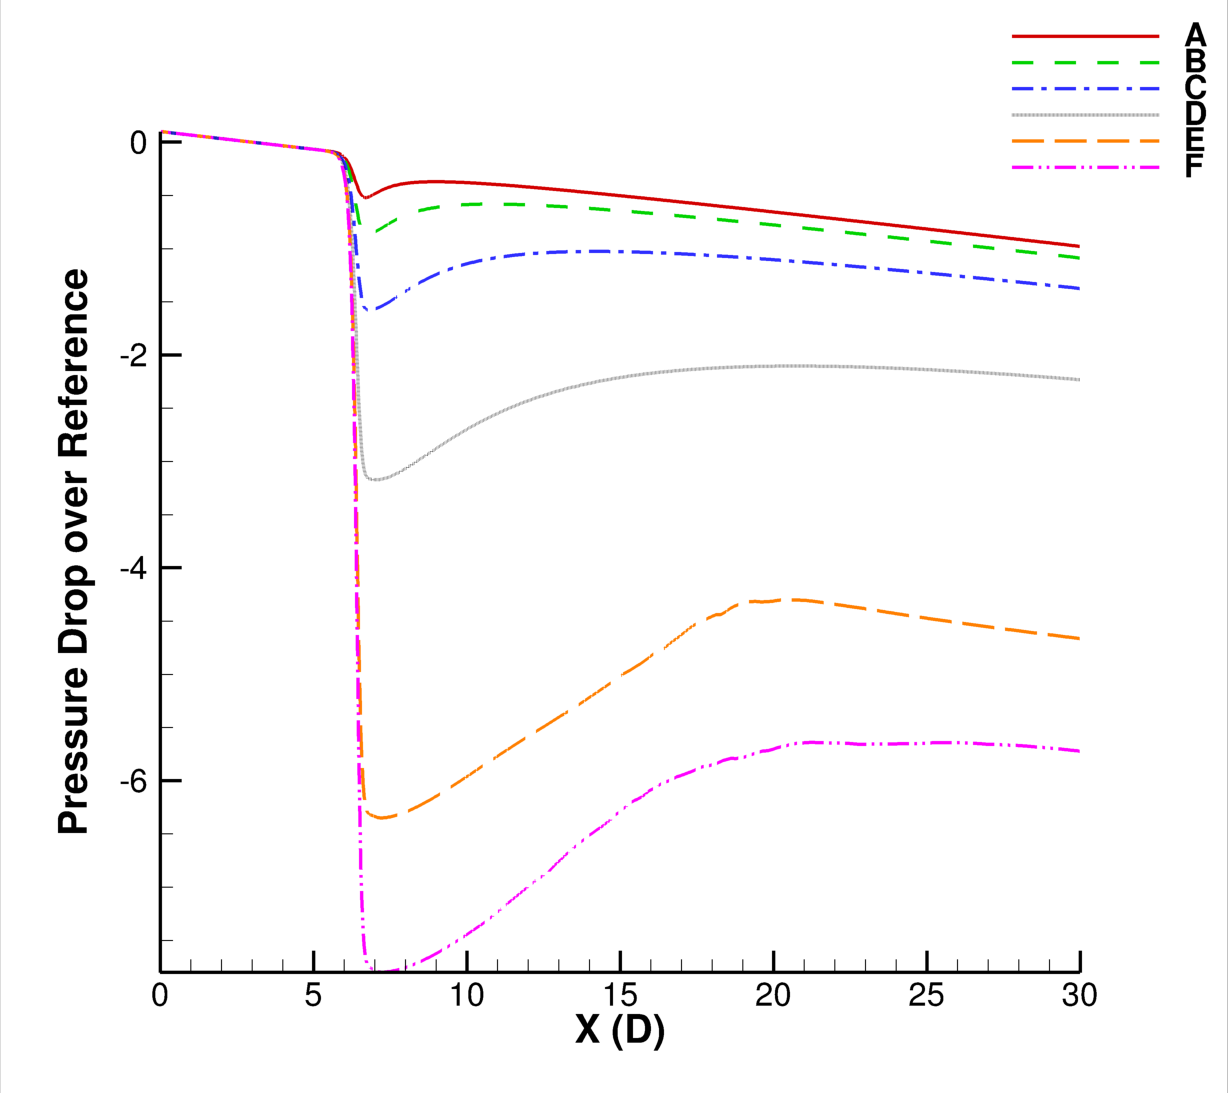
\includegraphics[trim= 1mm 0mm 1mm 0mm,clip,width=0.70\textwidth]{./pics/increase.png}
	\caption{Mean pressure drop of single stenosis for different blocking ratio}
	\label{fig:single increase}
\end{figure}

\begin{table}[h]
	\caption{Mean pressure drop of single stenosis for different blocking ratio}
	\vspace{-5pt}
	\begin{center}
		%	\scalebox{0.6}{
		\begin{tabular}{|c|c|c|c|}
			\hline
			\textbf{Cases} &\textbf{Degree} & \textbf{Streamwise PD} & \textbf{Absolute PD}\\
			\hline
			A & 40\% & 1.080 & 0.622\\
			\hline
			B & 50\% & 1.089 & 0.975\\
			\hline
			C & 60\% & 1.476 & 2.027\\
			\hline
			D & 70\% & 2.437 & 3.897\\
			\hline
			E & 78\% & 4.766 & 7.543\\
			\hline
			F & 80\% & 5.823 & 9.184\\
			\hline
		\end{tabular}
		%	}
	\end{center} 
\end{table}

\begin{figure}[H]
	\centering
	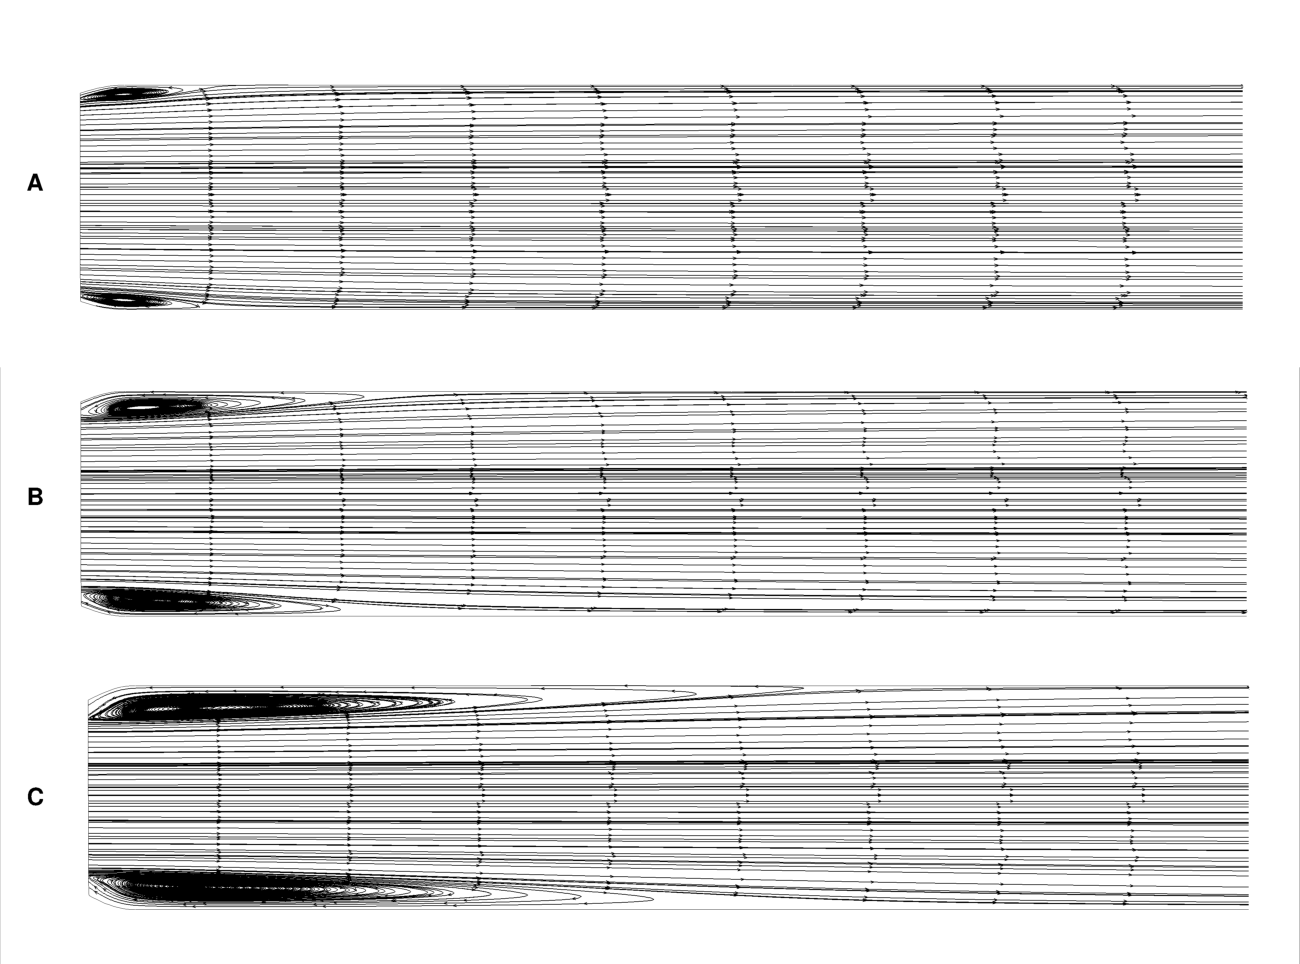
\includegraphics[trim= 1mm 1mm 1mm 0mm,clip,width=0.80\textwidth]{./pics/4to6.png}
	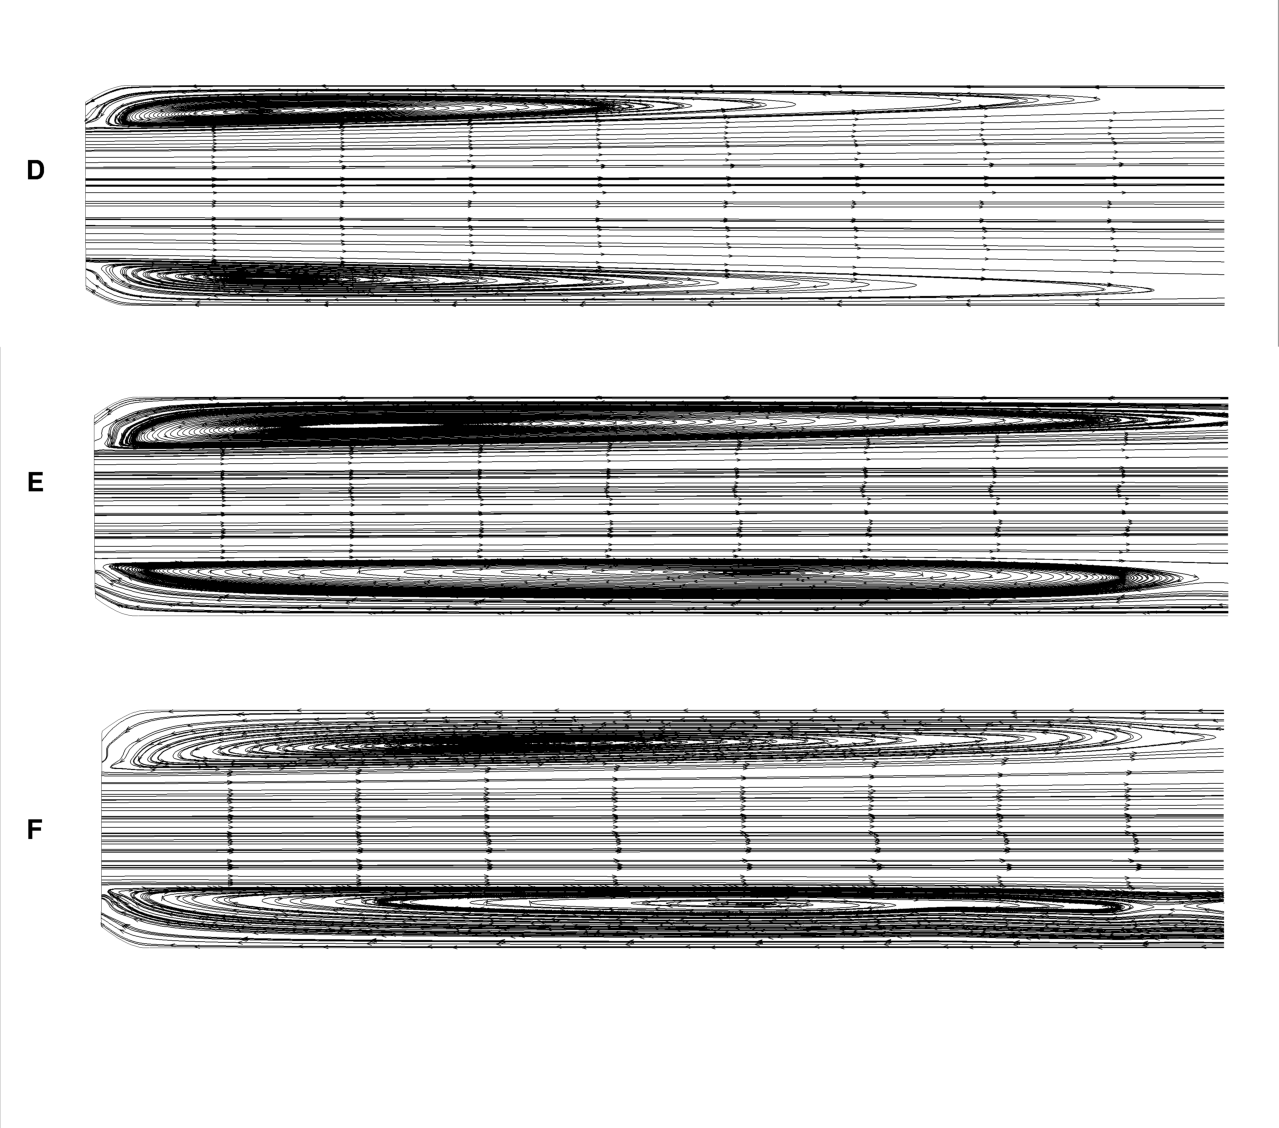
\includegraphics[trim= 1mm 0mm 1mm 0mm,clip,width=0.80\textwidth]{./pics/7to8.png}
	\caption{Single stenosis post-stenotic streamlines}
	\label{fig:single post streamlines}
\end{figure}

In Figure \ref{fig:single post streamlines},  we conduct a series simulations that range from 40\% to 80\% narrowing degree and plot the results on Figure \ref{fig:single increase} and Figure \ref{fig:single post streamlines}.
Figure \ref{fig:single increase} demonstrates the effects of single stenosis on the pressure drop from subcritical to critical regime. From the clinical perspective, when the area reduction ratio of stenosis is or over 60\%, it can be treated as a critical one. However, according to the above chart, the centreline pressure along streamwise direction decreases slowly in the unobstructed tube due to the wall shear stress. 
After the entrance tract, the pressure decreases significantly when the flow approaching to the stenotic region then slowly recovers past the narrowest cross-sectional area.
In the subcritical stenosis regime, the flow is mainly laminar, pressure fluctuation with decreasing and increasing is smooth and the scale is relative small.
When the degree of stenosis is more than 60\%, post-stenotic flow turns into transition, that produces large recirculation in the post-stenotic area.
The more severe narrowing degree leads to larger pressure drop and longer recovery length.
The above chart describes the detail of pressure distribution along streamwise direction and corresponds to the plot from empirical equation.

Figure \ref{fig:single post streamlines} presents the time-averaging both pressure field and velocity streamlines in the post-stenotic region. 
With the increasing of narrowing degree, the recirculation area increases and the pressure difference along the x direction becomes larger. 
From the case C to case D, the recirculation area grows rapidly.
Moreover, the plots of case E and case F show that their flow fields are unsteady.
As a result, when the narrowing degree is higher than 70\%, the constriction leads the original steady flow to unsteady stage.

\begin{figure}[H]
	\centering
	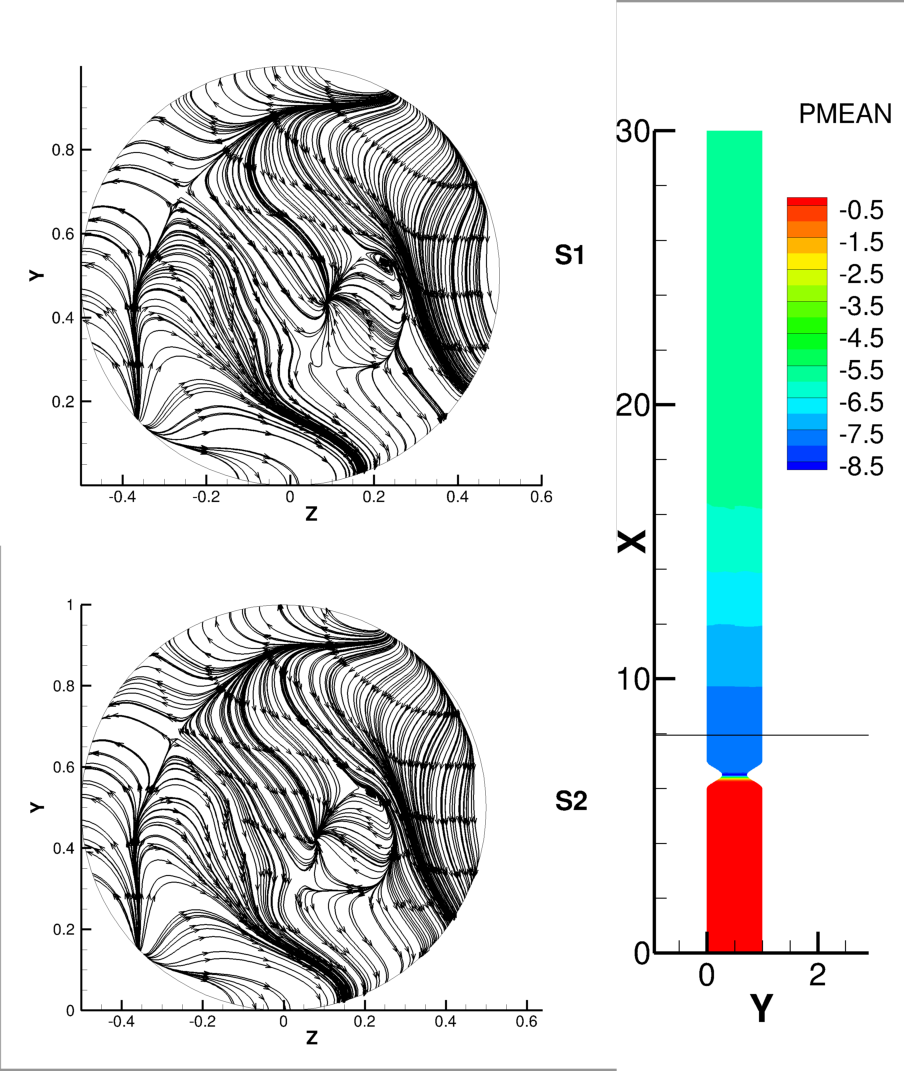
\includegraphics[trim= 1mm 1mm 1mm 1mm,clip,width=0.60\textwidth]{./pics/trans.png}
	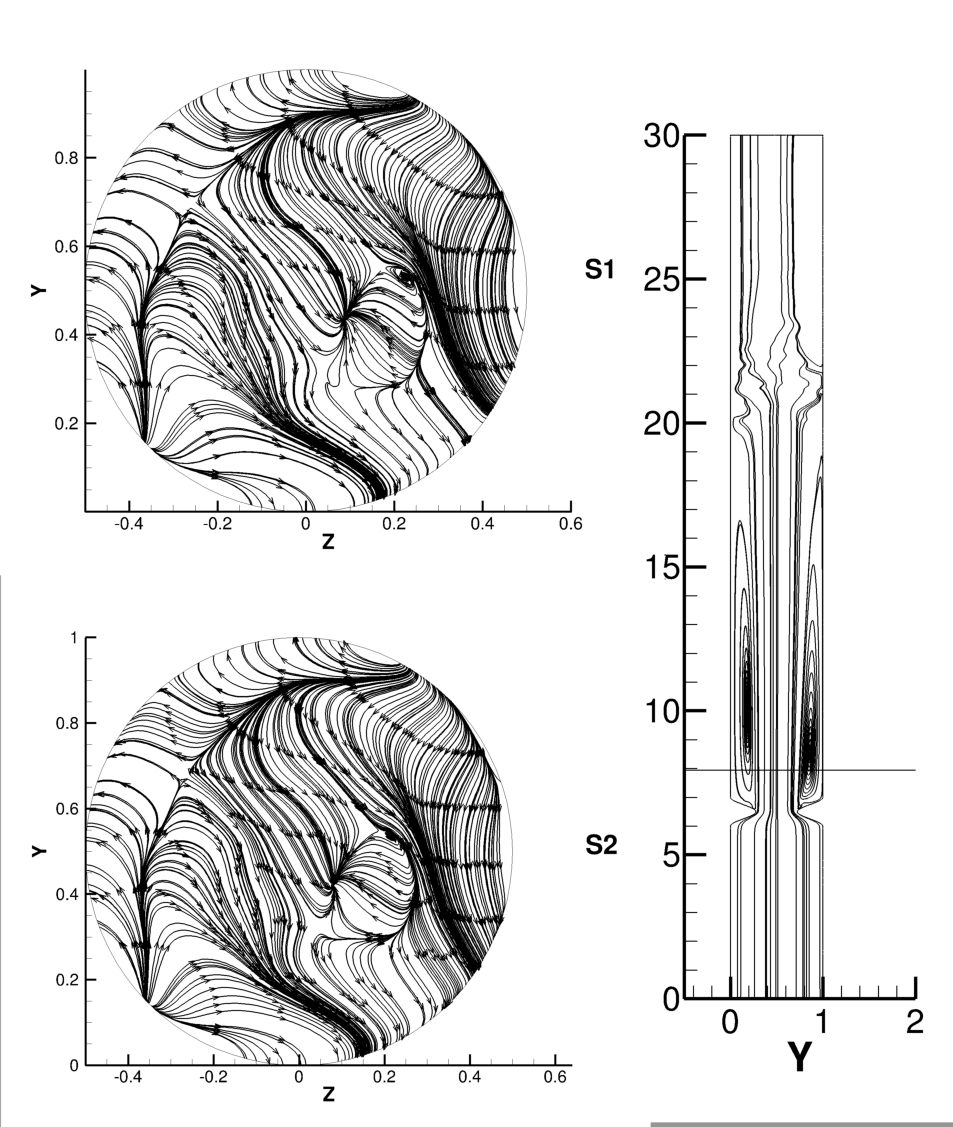
\includegraphics[trim= 1mm 2mm 1mm 1mm,clip,width=0.60\textwidth]{./pics/trans2.png}
	\caption{Stream line comparison in post-stenotic area}
	\label{fig:post streamline comparison}
\end{figure}

To verify the flow pass critical stenosis turns into highly unsteady flow. We present the streamline of both the transitional and time-averaging streamline plots of 80\% single stenosis in Figure \ref{fig:post streamline comparison}.
In the downstream region, the recirculation exists as the length of 8-10 diameters along streamwise direction.
After the recirculation region, the time-averaging streamlines are smoothly going to the outlet while the transitional streamlines are curvature and circuitous.
This comparison indicates that the flow passing critical stenosis is unsteady. 
Meanwhile, the recirculation region streamwise length corresponds to the pressure recovery length.\\

The clinical criterion between subcritical and critical stenosis is varying from 60\% to 75\% narrowing degree.
This criterion is a practical guidance for doctors making decisions on occlusive disease treatment.
From the hemodynamic perspective, the non-laminar flow may cause endothelial dysfuction and increased thrombogenicity.
For the healthy femoral arteries, the Reynolds number of blood flow is around 500. 
The stenosis accelerates flow speed and increases the Reynolds number.
For flow in pipe of diameter $D$, experimental observations show that the laminar flow occurs when $Re_D < 2300$.
The following Reynolds number equation can predict the flow pattern in stenotic area:


\begin{equation}
Re = \frac{\textbf{Q} D_H}{\nu A}
\end{equation}
where $\textbf{Q}$ is the volumetric flow rate, $A$ is the pipe cross-sectional area, $\nu$ is kinematic viscosity
and $D_H$ is the diameter.
If the flow pass 50\% diameter reduction (correspondingly 75\% area reduction) stenosis, the Reynolds number increases from 500 to 1000.

According to our single stenosis simulation results in Figure \ref{fig:single post streamlines} and Figure \ref{fig:post streamline comparison}, when the narrowing degree is over 70\%, the post-stenotic flow unsteadiness increases significantly. Also, the recirculation area grows rapidly with the narrowing degree increasing.

In between case D and case F, we insert one 78\% stenosis as case E. Although the difference of area narrowing degree between case E and case F is only 2\%, the streamwise PD and absolute PD increase by 22.18\% and 21.76\%. When the narrowing degree is over the critical threshold, even slight magnitude change causes significant effect on flow field.
The growth of pressure drop is not linear to the narrowing changing.  
For general stenotic cases, the definition of critical stenosis depends on variant flow condition. 
We present the CFD simulation which has the capability to predict the flow field and find out specific critical stenosis threshold.

\subsection{Pressure drop between multiple sub-critical stenoses and single critical stneosis}

\begin{figure}[H]
	\centering
	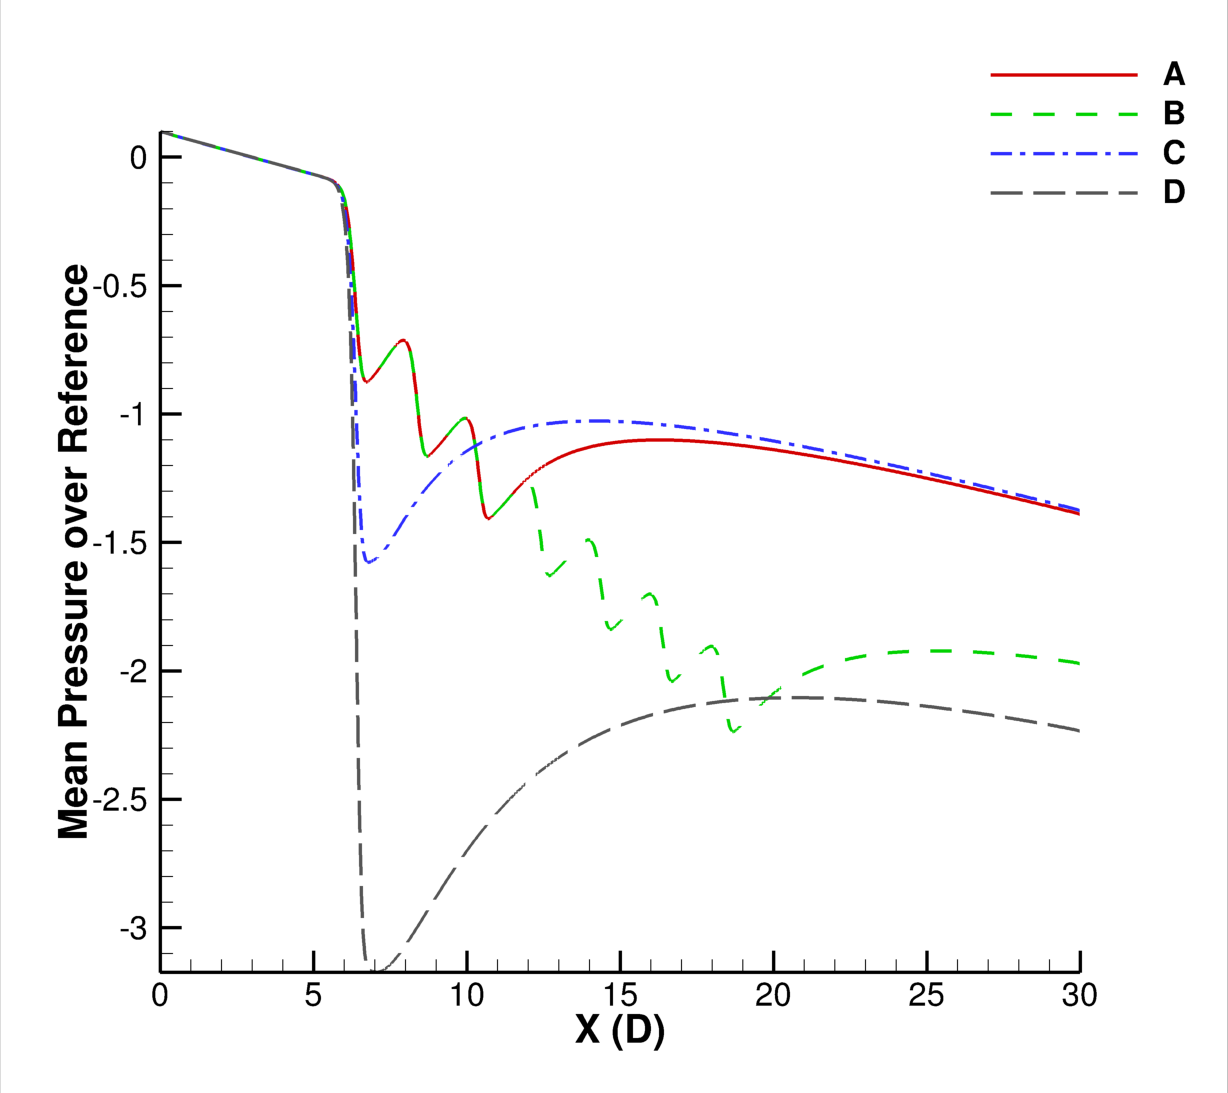
\includegraphics[trim= 1mm 1mm 1mm 1mm,clip,width=0.60\textwidth]{./pics/newcomp.png}
	\caption{Pressure drop among multiple subcritical stenoses}
	\label{fig: pressure drop among multiple subcritical stenoses}
\end{figure}

\begin{table}[h]
	\caption{Pressure drop among multiple subcritical stenoses}]
	\label{Table: pressure drop among multiple subcritical stenoses}
	\vspace{-5pt}
	\begin{center}
		%	\scalebox{0.6}{
	 \begin{tabular}{|c|c|c|c|}
	 	\hline
	 	\textbf{Cases} &\textbf{Degree} & \textbf{Streamwise PD} & \textbf{Absolute PD}\\
	 	\hline
	 	A & Three 50\% & 1.471 & ---\\
	 	\hline
	 	B & Seven 50\% & 2.387 & ---\\
	 	\hline
	 	C & Single 60\% & 1.476 & 2.027\\
	 	\hline
	 	D & Single 70\% & 2.437 & 3.897\\
	 	\hline
	 \end{tabular}
		%	}
	\end{center} 
\end{table}

In Figure \ref{fig: pressure drop among multiple subcritical stenoses} and Table \ref{Table: pressure drop among multiple subcritical stenoses},  we can find that the streamwise pressure drop of three and seven subcritical (50\%) stenoses is higher than the pressure drop introduced by single critical (60\%) stenosis (Figure 8). 
Therefore, the assumption of multiple sequential subcritical stenosis produces more pressure drop than single critical stenosis is proved by quantitative plot. 
We find that the pressure drop of both three 50\% stenoses and one single 60\% stenosis is closer while the flow propagating towards to the outlet, that because of the length of control vessel plays a non-neglectable role when we deciding the pressure drop difference.
The pressure plot clearly illustrates pressure recovery region then we can put the check point out of that section.
We also noticed that the absolute pressure drop of one single 60\% stenosis is higher than that of any 50\% stenoses. 
The more severe absolute pressure drop of critical stenosis introduces more unpleasant hemodynamic effect on vessels such as the larger wall shear stress applied on post-stenotic tube walls. 

\subsection{Multiple critical stenoses analysis}

\begin{figure}[H]
	\centering
	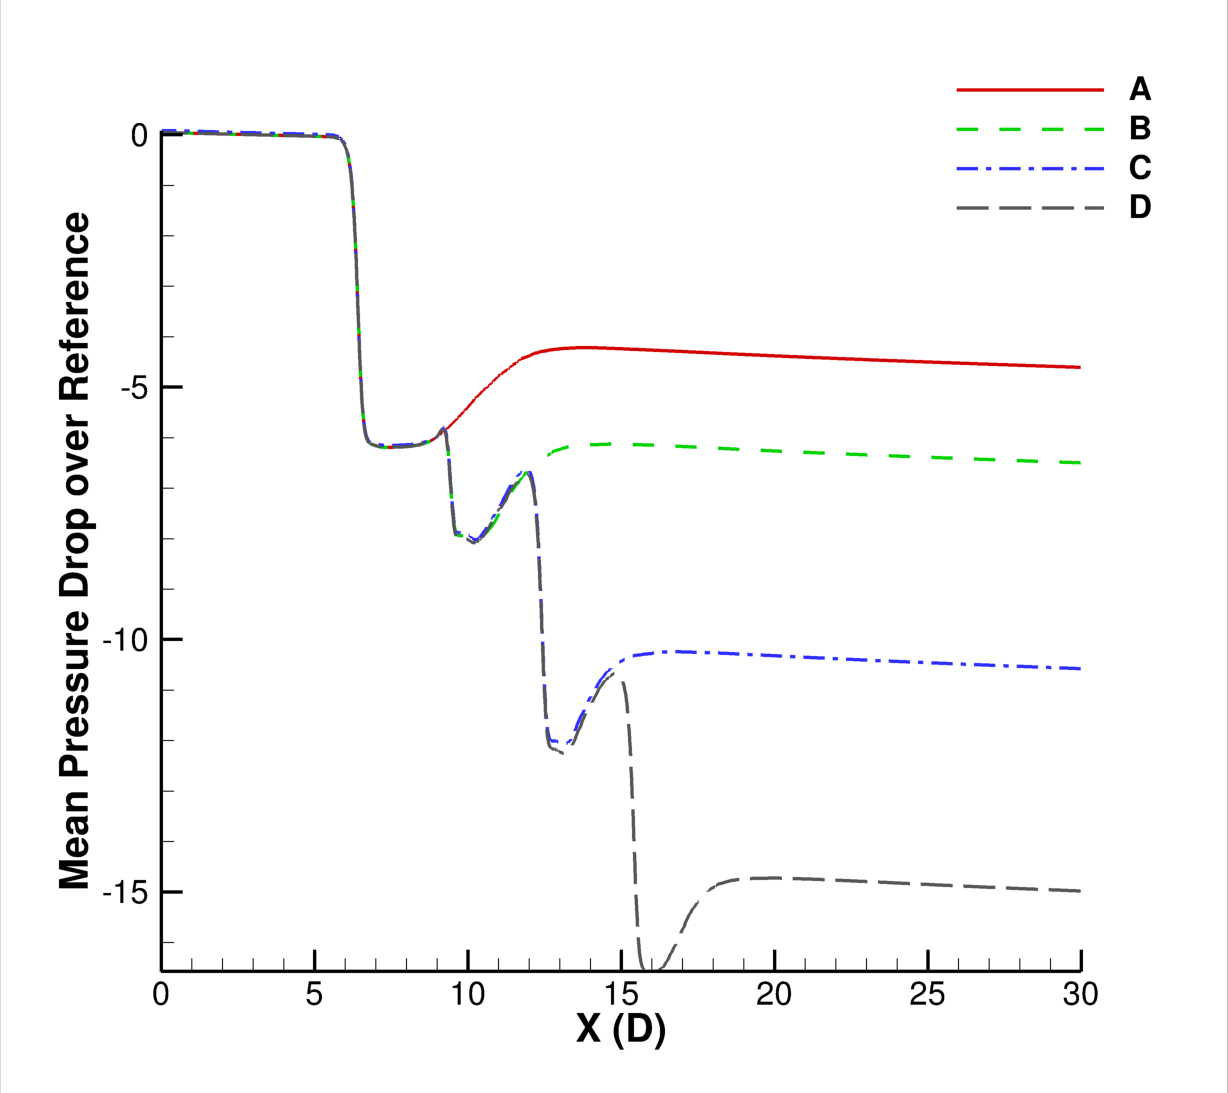
\includegraphics[trim= 1mm 0mm 1mm 0mm,clip,width=0.60\textwidth]{./pics/exper.png}
	\includegraphics[trim= 1mm 0mm 1mm 0mm,clip,width=0.60\textwidth]{./pics/Graph1.png}
	\caption{Pressure drop among multiple critical stenoses}
	\label{fig: Pressure drop among multiple critical stenoses}
\end{figure}

In Figure \ref{fig: Pressure drop among multiple critical stenoses}, for very critical stenoses, such as $ 78\% $ area deduction, the blood through stenotic area is into the transition stage. The error between simulation and experiments is less than $ 20\% $. We have legit results in simulation. Furthermore, we can find the pressure drop is linearly proportional to the number of critical stenoses. The scale of pressure drop is close to $ 15 $ times of the regular inlet pressure which means a significant pressure and recirculation damage is caused upon the post-stenotic region. Now we also proved the dangerousness of multiple critical stenoses along the artery.


%========================================================
\subsection{Multiple subcritical stenoses pressure drop}

\begin{figure}[H]
	\centering
	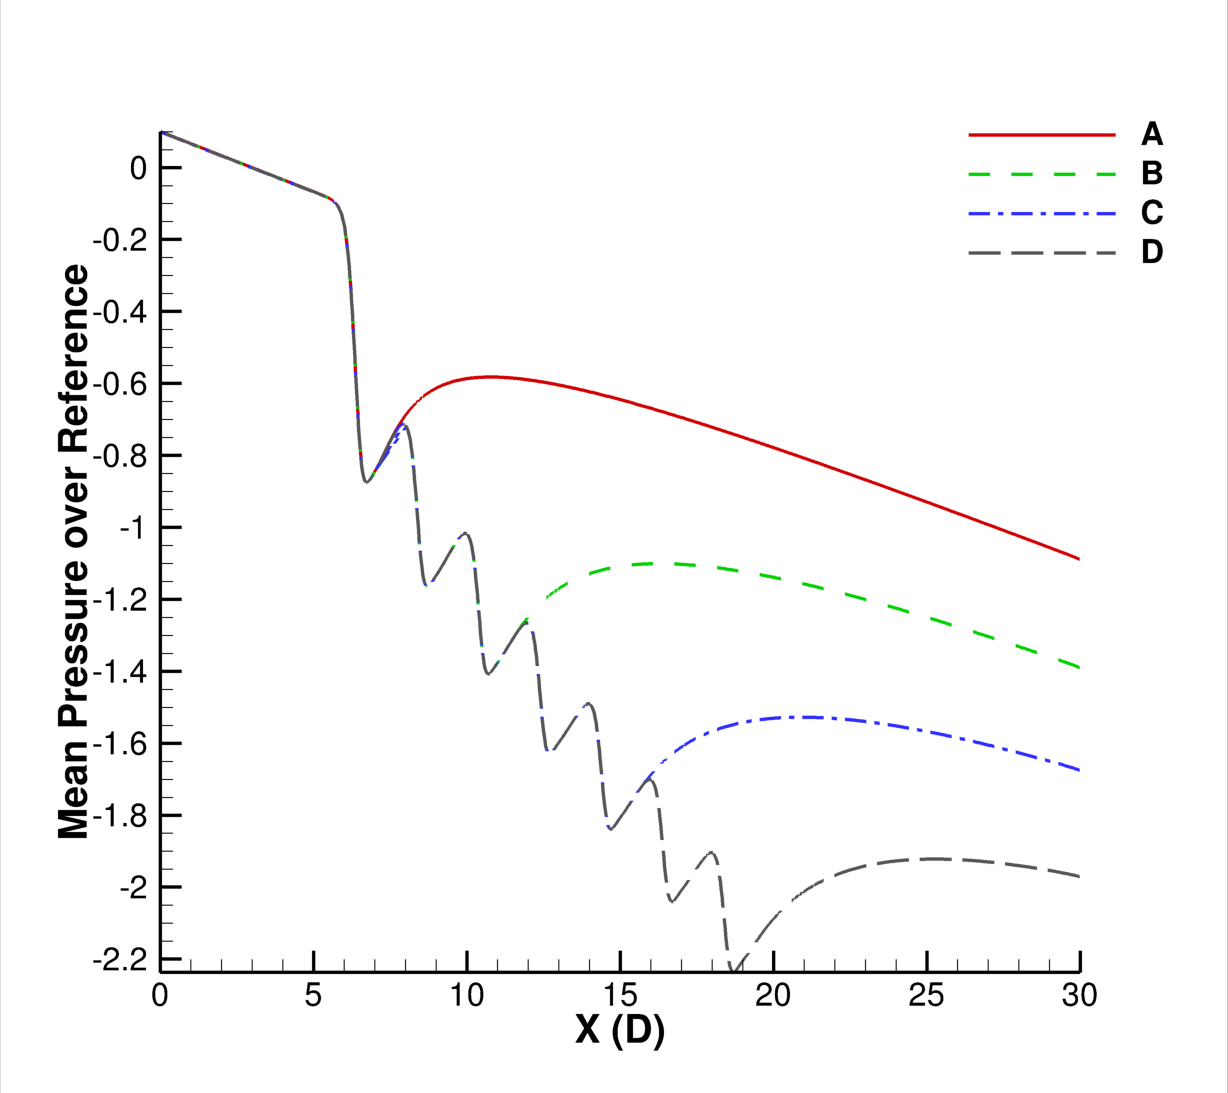
\includegraphics[trim= 1mm 0mm 1mm 0mm,clip,width=0.60\textwidth]{./pics/m50.png}
	\caption{Pressure drop among multiple subcritical stenoses}
	\label{fig: Pressure drop among multiple subcritical stenoses}
\end{figure}

\begin{figure}[H]
	\centering
	\includegraphics[width=0.60\textwidth]{./pics/multi50.png}
	\caption{Pressure drop values of multiple subcritical stenoses}
	\label{fig:Pressure drop values of multiple subcritical stenoses}
\end{figure}


The effect of adding subcritical stenoses onto the same vessel is not well discussed yet. 
We simulate the 50\% degree subcritical stenosis and then sequentially add same stenosis to the downstream region. The maximum number is seven. We plot the pressure drop of one, three, five and seven stenoses along the centerline.  
The Figure \ref{fig: Pressure drop among multiple subcritical stenoses} shows the pressure drop increasing with more stenoses applied on the same straight tube.
The following added stenoses do not have the effect on the upstream stenoses flow field. The effect on pressure drop and pressure recovery area are similar for each constriction.
For the right figure, we deduct the pressure drop of non-obstructed tube ,which only generated from wall shear stress, from the total stream-wise pressure drop. 
We plot the net pressure drop from non-obstruction to seven subcritical stenoses correspondingly.
The plot on right figure demonstrates the linear increasing of net pressure drop versus the increasing number of applied stenoses.
The linear net pressure drop increasing is an important feature of subcritical stenoses.

\subsection{Stenosis stretching on streamwise direction}

\begin{figure}[H]
	\centering
	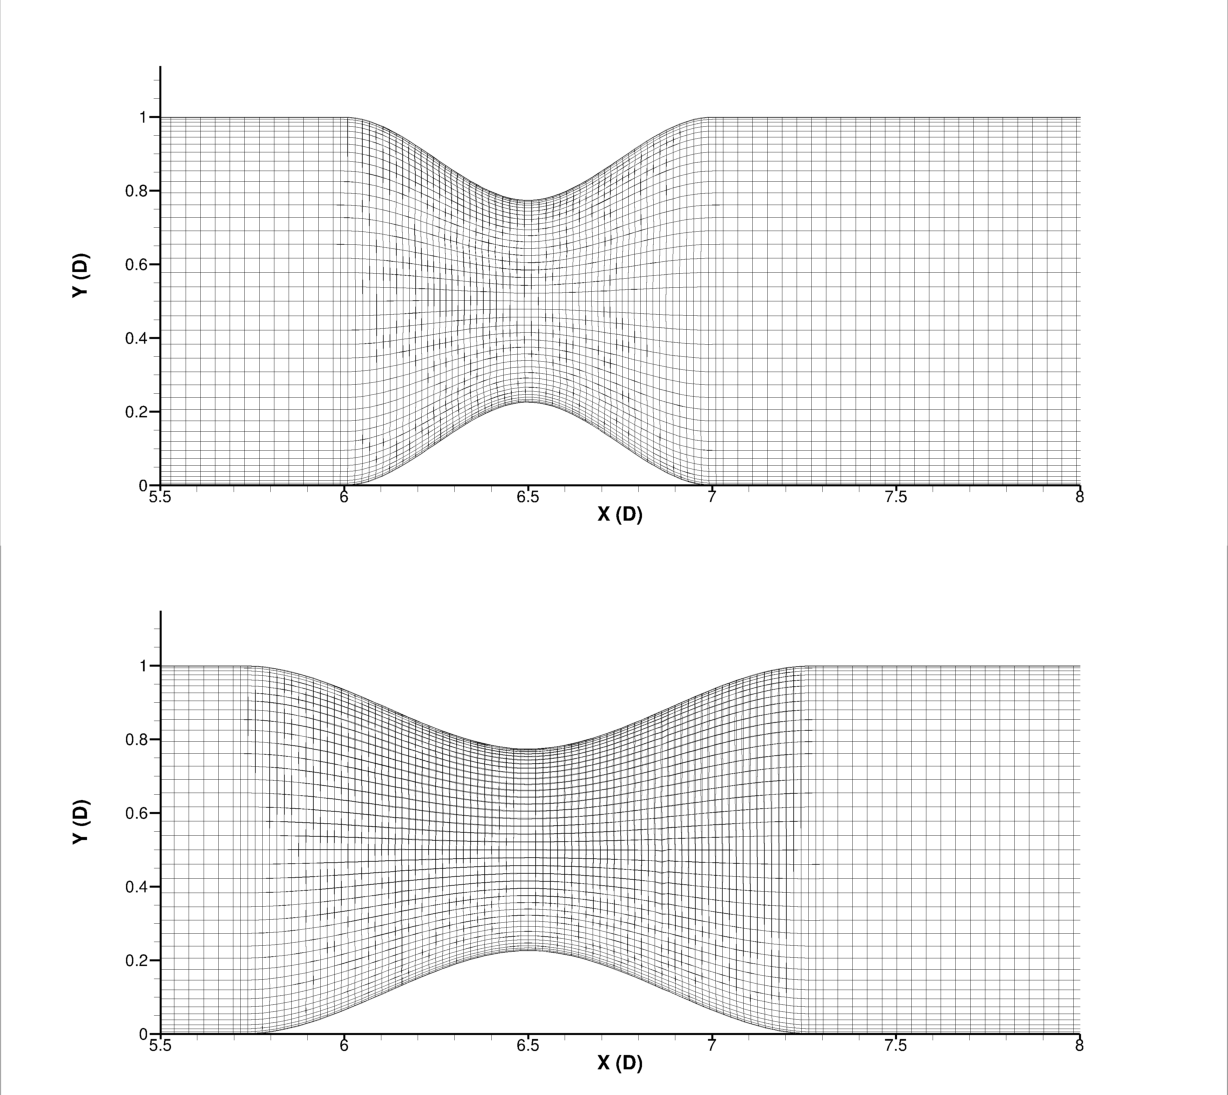
\includegraphics[trim= 1mm 0mm 0mm 0mm,clip,width=0.60\textwidth]{./pics/meshes.png}
	\caption{Mesh along original and deformed stenotic region.}
	\label{fig:Mesh along original and deformed stenotic region}
\end{figure}

\begin{figure}[H]
	\centering
	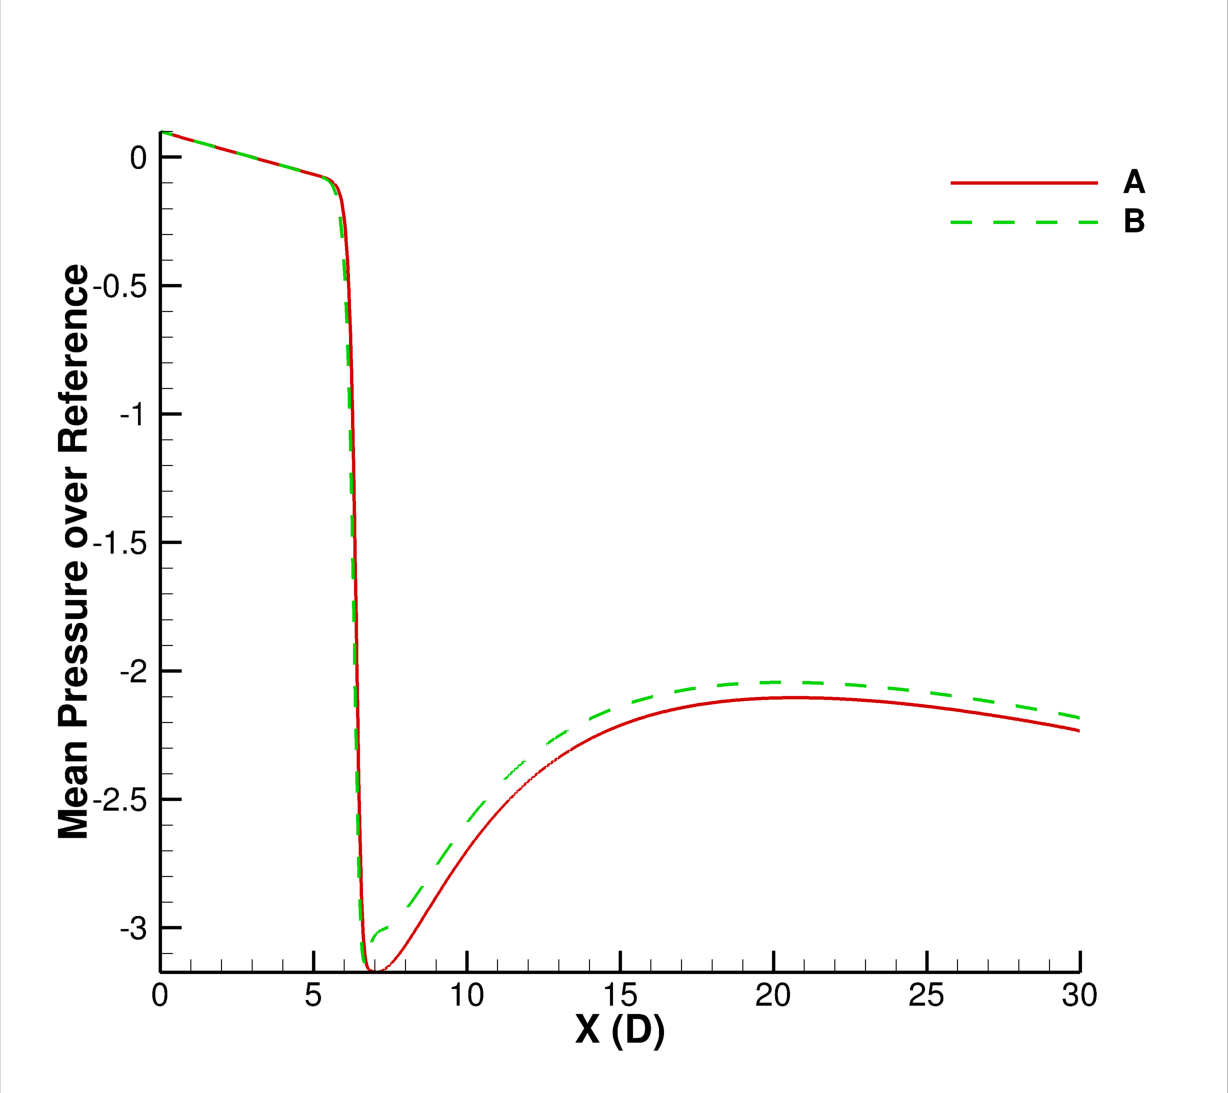
\includegraphics[trim= 1mm 0mm 1mm 0mm,clip,width=0.60\textwidth]{./pics/deform.png}
	\caption{Pressure drop comparison between original and deformed stenosis.}
	\label{fig:Pressure drop comparison between original and deformed stenosis}
\end{figure}

\begin{figure}[H]
	\centering
	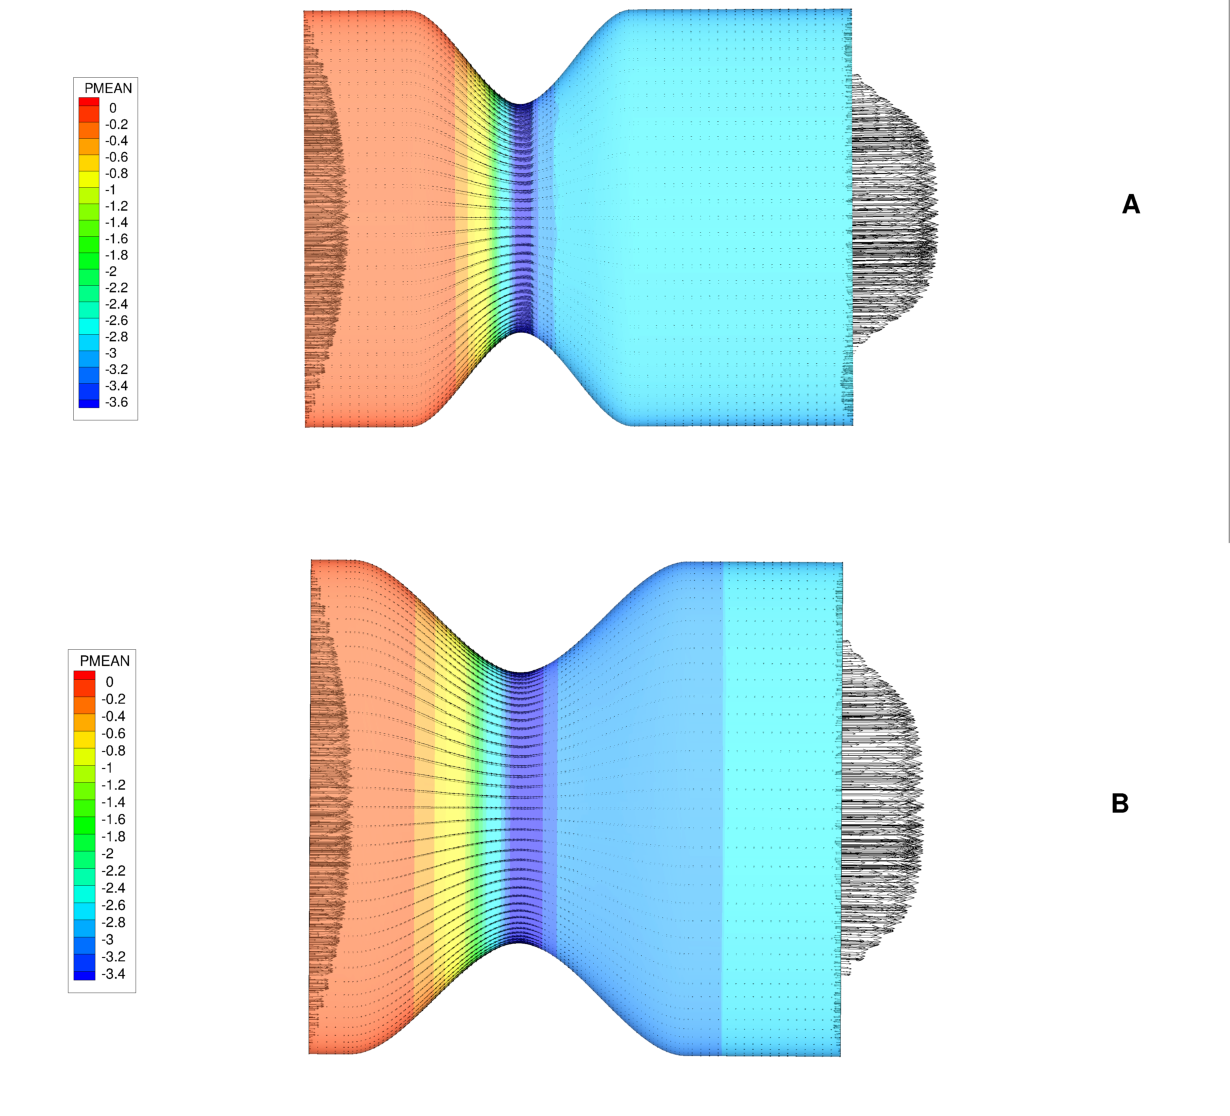
\includegraphics[trim= 1mm 0mm 0mm 0mm,clip,width=0.60\textwidth]{./pics/deform2.png}
	\caption{Streamlines along original and deformed stenosis.}
	\label{fig:Streamlines along original and deformed stenosis}
\end{figure}


\begin{table}[h]
	\caption{Pressure drop comparison between original and deformed stenosis.}
	\label{Table: Pressure drop comparison between original and deformed stenosis}
	\vspace{-5pt}
	\begin{center}
		%	\scalebox{0.6}{
		\begin{tabular}{|c|c|c|c|}
			\hline
			\textbf{Cases} &\textbf{Degree} & \textbf{Streamwise PD} & \textbf{Absolute PD}\\
			\hline
			A & Original 70\% & 2.437 & 3.897\\
			\hline
			B & Stretched 70\% & 2.284 & 3.742\\
			\hline
		\end{tabular}
		%	}
	\end{center} 
\end{table}


We deform the shape of 70\% degree stenosis by stretching it on streamwise direction, see Figure \ref{fig:Mesh along original and deformed stenotic region}.
We elongate the stenotic region and maintain the narrowest cross-sectional area size.
The above chart demonstrates the meshes comparison of two shapes of stenosis and the centerline pressure drop along streamwise direction.
The streamwise length of the stenosis is increased by 54\% while the corresponding pressure drop is only decreased by 1.8\%.
With the stretching of stenosis, the smoother narrowing curvature leads to the slightly more pressure recovery which is identified on the right chart ranges from 7D to 15D along the x axis, in Figure \ref{fig:Pressure drop comparison between original and deformed stenosis} and Table \ref{Table: Pressure drop comparison between original and deformed stenosis}.
The streamwise pressure drop is decreased due to the smoother stenotic curve while the absolute pressure drop remains the same level since the narrowing degrees are still the same for both cases.
We can conclude that the longitudinal shape of single stenosis plays a minor role in the hemodynamic effect on flow pass stenosis.
Moreover, the narrowing degree is the main factor which dominates the scale of total streamwise pressure drop across the constriction.

%===================================================================================

\subsection{Pressure drop and wall shear stress}
\begin{figure}[H]
	\centering
	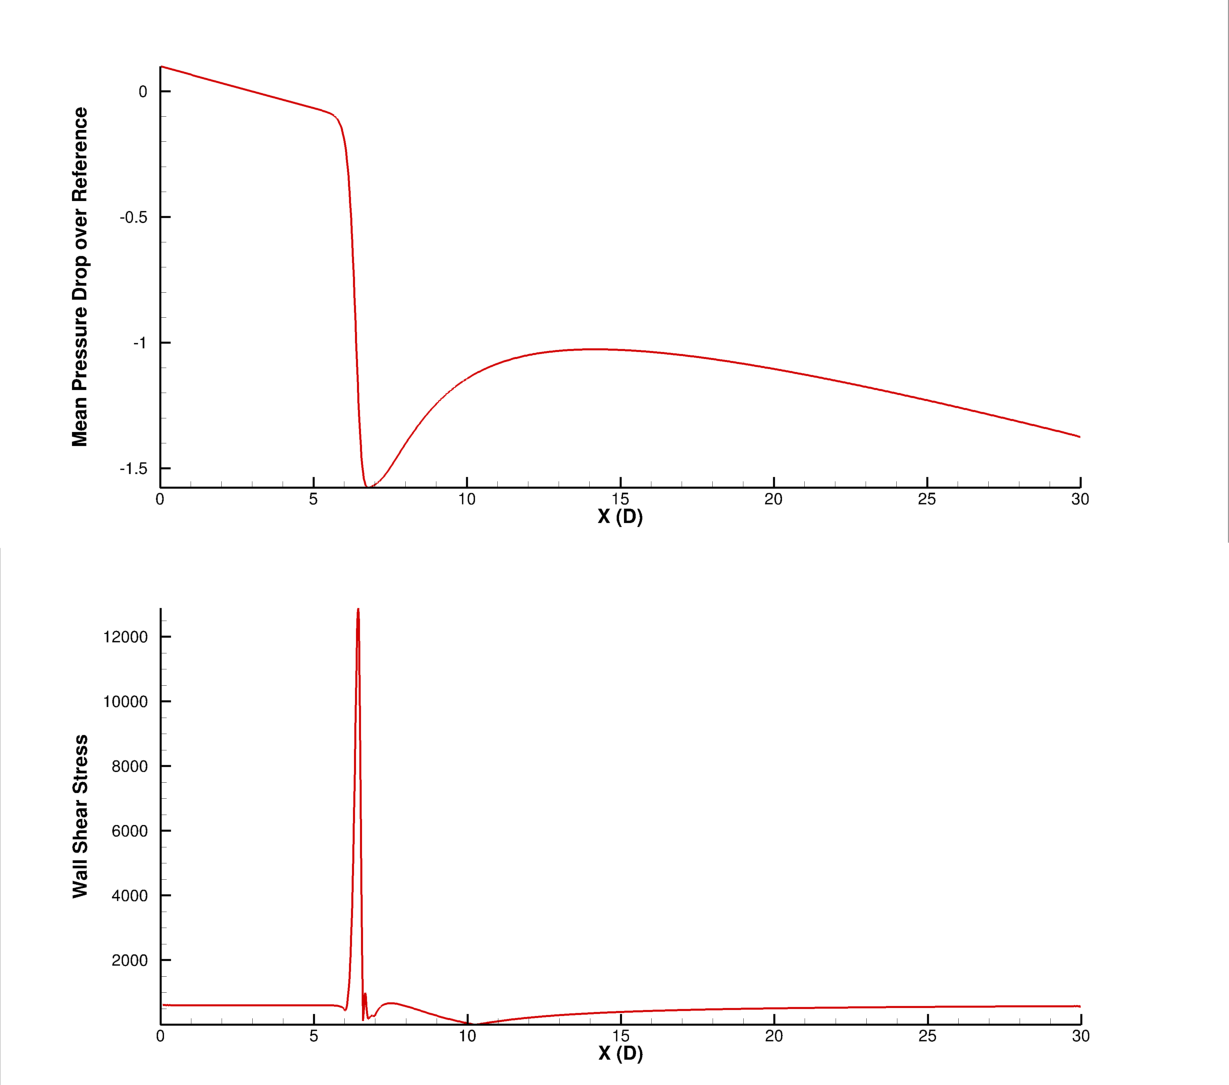
\includegraphics[trim= 1mm 0mm 1mm 0mm,clip,width=0.60\textwidth]{./pics/pandws.png}
	\caption{Pressure drop and wall shear stress across single critical stenosis}
	\label{fig:pandws}
\end{figure}

In Figure \ref{fig:pandws}, we plot the pressure and wall shear stress along streamwise direction of single 60\% stenosis case.
The highest wall shear stress corresponds to the lowest pressure which happened at slightly pass the center of stenosis.
For the wall shear stress chart, after the peak point, the plot tend close to the x-axis twice. 
The recirculation region is between the two lowest points.
After the narrowest cross-sectional area, the pressure recovers smoothly while the shear stress fluctuates due to the post-stenotic recirculation.

%===================================================================================

\subsection{Interval spacing between subcritical stenoses}

\begin{figure}[H]
	\centering
	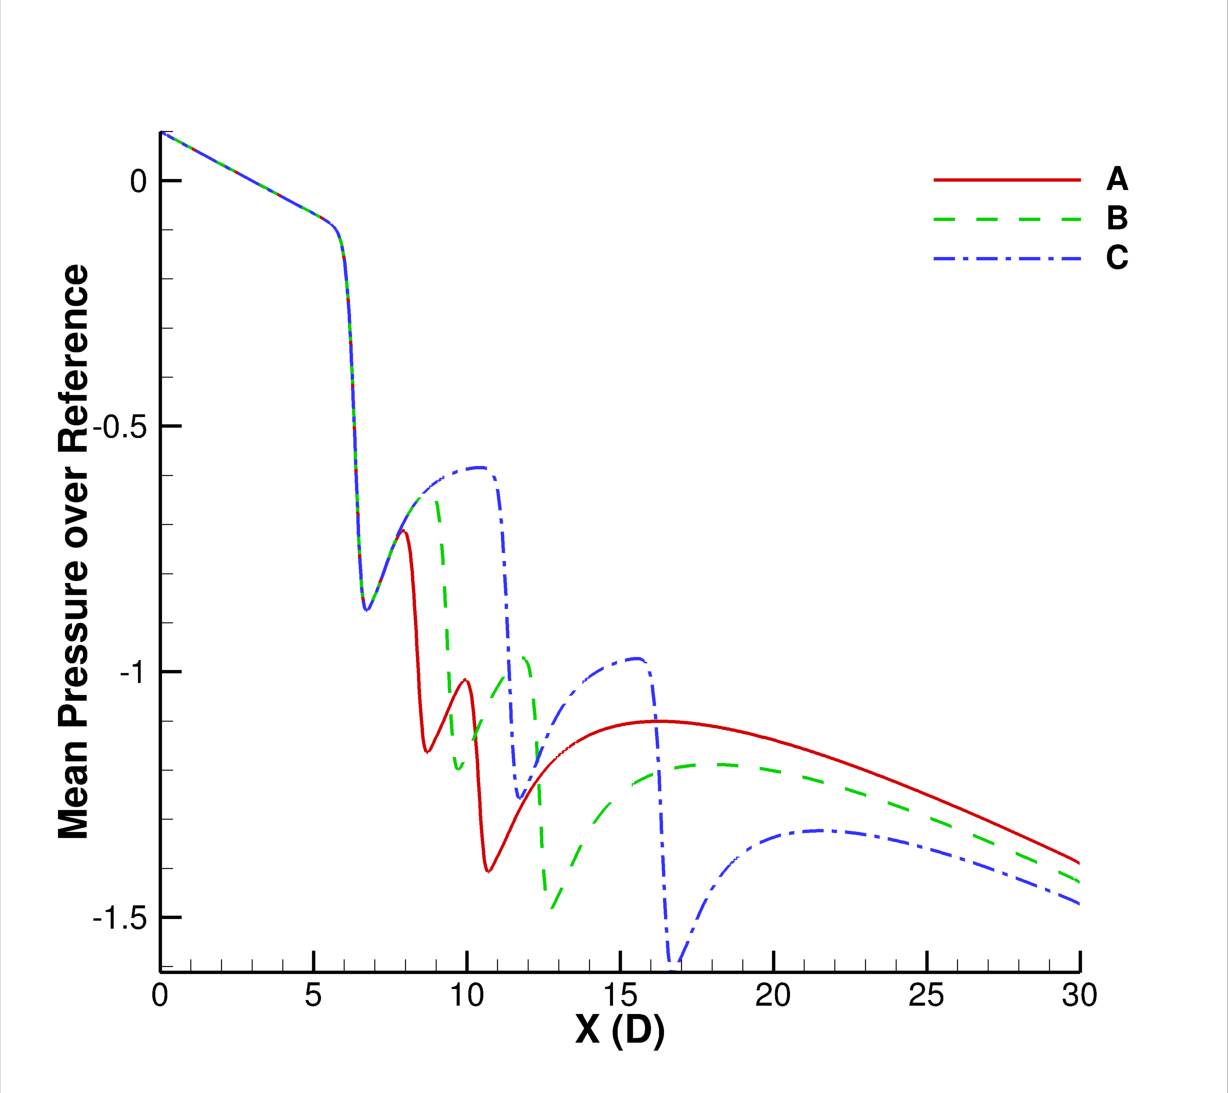
\includegraphics[trim= 1mm 0mm 1mm 0mm,clip,width=0.60\textwidth]{./pics/interval.png}
	\caption{Pressure drop of different interval spacing.}
	\label{fig:Pressure drop of different interval spacing}
\end{figure}

\begin{figure}[H]
	\centering
	\includegraphics[width=0.60\textwidth]{./pics/pvsinterval.png}
	\caption{Pressure drop values of different interval spacing.}
	\label{fig:Pressure drop values of different interval spacing}
\end{figure}

\begin{table}[h]
	\caption{Pressure drop of different interval spacing.}
	\label{Table: Pressure drop of different interval spacing}
	\vspace{-5pt}
	\begin{center}
		%	\scalebox{0.6}{
		\begin{tabular}{|c|c|c|c|}
			\hline
			\textbf{Cases} &\textbf{Degree} & \textbf{Streamwise PD} & \textbf{Absolute PD}\\
			\hline
			A & One time spacing & 1.49 &1.51\\
			\hline
			B & Two times spacing & 1.53 &1.58\\
			\hline
			C & Four times spacing & 1.57 &1.71\\
			\hline
		\end{tabular}
		%	}
	\end{center} 
\end{table}


The patient specific stenoses structure is highly complicated with lots of uncertain variables. 
The interval spacing between adjacent stenoses is an important parameter.
To our best knowledge, few studies have been conducted on this perspective.
Among previous the models that we created, I set same spacing between adjacent sub-critical stenoses which is one diameter for the sake of consistency. 
However, from the Figure \ref{fig: patient CT} we find that along the patients' peripheral artery, the spacing is significantly larger than one diameter. 
To reveal how the pressure drop changing with interval spacing increasing, we operate a series of simulations which ranges the interval spacing from 1D to 4D in Figure \ref{fig:Pressure drop of different interval spacing} and Table \ref{Table: Pressure drop of different interval spacing}. 
The comparison included interval spacing of one, two and four times of diameter for sub-critical stenoses.  
Both streamwise pressure drop and absolute pressure drop developed with spacing increasing. 
We can also see from the chart that the incline slope is not significant. 
Although the spacing increased from 1 to 4, the pressure drop growth is 16\% and 14\% referring to streamwise pressure drop and absolute pressure drop respectively.  


%===================================================
\section{Summary and discussion}
According to the data and figures, we proved our following predictions:
The post-stenotic flow becomes highly unsteady when the narrowing degree is more than 60\%.
More than 3 50\% stenoses cause more streamwise pressure drop than one single 60\% stenosis.
Pressure drop introduced by subcritical stenoses grows almost linear as the increasing number of applied stenoses. 
Cross-sectional area reduction is the main factor which contributes to the total. The streamwise length of stenosis has little effect on the flow field.
The interval spacing between each stenoses has small contribution to the total pressure drop.


With the our promising results and effective solver, we have built up a solid foundation for multiple stenoses research. The next step will be patient-specific geometry investigation. The high fidelity results are good supplement for doctors diagnosis leading to best optimized treatment strategy.   